% ***************************************************************
%   MASS IN HONOR OF THE SOLEMNITY OF CHRIST KING OF THE UNIVERSE
%   Music and accompaniment by serachsam
% ***************************************************************

% - Preambulo
\documentclass[12pt, letterpaper]{report}

%%% - Paquetes
\usepackage[utf8]{inputenc}
\usepackage[T1]{fontenc}
\usepackage{xcolor}
\usepackage{pifont}
\usepackage{lettrine}
\usepackage{lmodern}
\usepackage{enumitem}
% Utilizamos el paquete para gestionar imagenes jpg
\usepackage{graphicx}
\graphicspath{ {../images/} }

\oddsidemargin -1.0cm
\headsep -1.0cm
\textwidth=18.5cm
\textheight=23cm

\setlength{\parskip}{\baselineskip}

\setcounter{secnumdepth}{0}
\setcounter{tocdepth}{4}

%% Portada del Libro
\title{
  \textbf{ \Huge Misa Cristo Rey  } \\
  { \LARGE Solemnidad Cristo Rey del Universo } \\
  \vspace{2em}
  
\includegraphics{logo}
}

\author{ \textit{ \large Carmelitas Descalzas, Managua, Nicaragua } }

\date{ \Large \textbf{Linda Isabel Mart\'inez Castro \\ Samuel Jos\'e Guti\'errez Avil\'es} \\ \small \textit{2018 - 2020} }

%Empieza el documento %%%%%%%%%%%%%%%%%%%% P R I N C I P I O %%%%%%%%%%%%%%%%%%%%%%%%%%%%%%
\usepackage{graphics}
\begin{document}
    %% - Portada
    \maketitle

    %% - Indice
    \LARGE ÍNDICE GENERAL

    \large \hfill{Página}\\
    \Large \textbf{Introducción \hfill{2}}\\
    .\hspace{1cm} \large Historia \dotfill 3\\
    .\hspace{1cm} \large Estructura de la Misa \dotfill 4\\
    .\hspace{1cm} \large Ordinario \dotfill 6\\
    .\hspace{1cm} \large Propio \dotfill 6

    \noindent
    \Large \textbf{Ordinario de la Misa \hfill{9}}\\
    .\hspace{1cm} \large Señor ten piedad \dotfill 10\\
    .\hspace{1cm} \large Gloria a Dios en lo alto del cielo \dotfill 16\\
    .\hspace{1cm} \large Credo \dotfill 26\\
    .\hspace{1cm} \large Santo \dotfill 39\\
    .\hspace{1cm} \large Cordero de Dios \dotfill 48

    \noindent
    \Large \textbf{Propio de la Misa \hfill{57}}\\
    .\hspace{1cm} \large Canto de Entrada \dotfill 58\\
    .\hspace{1cm} \large Salmo Responsorial \dotfill 69\\
    .\hspace{2cm} \large \textit{Ciclo A} \dotfill 69\\
    .\hspace{2cm} \large \textit{Ciclo B} \dotfill 79\\
    .\hspace{2cm} \large \textit{Ciclo C} \dotfill 86\\
    .\hspace{1cm} \large Aleluya \dotfill 93\\
    .\hspace{1cm} \large Presentación de Ofrendas \dotfill 98\\
    .\hspace{1cm} \large Canto de Comunión \dotfill 112\\
    .\hspace{1cm} \large Canto de Despedida \dotfill 122
    \clearpage

    %% - Introduccion
    \begin{center}
        \vspace*{9cm}
        \textbf{\Huge Introducci\'on}
    \end{center}
    \clearpage

    \LARGE HISTORIA

    \Large La composici\'on de la ``Misa Cristo Rey'' para la solemnidad del mismo nombre fue realizada en varias etapas, empezando en el a\~no 2018. La realizaci\'on de la obra empez\'o luego de varias platicas con las hermanas Carmelitas Descalzas del Crucero, Managua, quienes nos hab\'ian hecho ya algunas solicitudes de piezas para diversas ocasiones. Acerc\'andose la solemnidad de Cristo Rey del Universo de ese a\~no, una de las hermana nos menciono la posibilidad de componer una pieza dedicada a la Madre del monasterio, la cual en esa \'epoca era la hermana Carmen Teresa de Cristo Rey, en honor a su nombre espiritual y de la solemnidad. Esa pieza nunca se concluyo, pero en cambio nos animo a investigar sobre la existencia de m\'usica dedicada a esa solemnidad; durante la investigaci\'on nos dimos cuanta que exist\'ian algunas piezas sueltas dedicadas a Cristo Rey pero nada completo, y decidimos realizar una obra completa para Cristo Rey del Universo la cual nos llevo tres a\~nos para poderla finalizar.

    A finales del 2019, luego de pasar por diversos estilos musicales y varios intentos, solo ten\'iamos terminado el ordinario de la misa, acerc\'andose la solemnidad de Cristo Rey de Universo de ese a\~no se imprimi\'o y entrego a las hermanas Carmelitas Descalzas con una dedicatoria a la Hna. Carmen Teresa de Cristo Rey, quien ya hab\'ia dejado de ser la Madre del monasterio. Finalizada y entregada la misa con solo el ordinario, nos dimos cuenta que la misa como forma musical propone m\'as que solo el ``Kyrie eleison'', ``Gloria in excelsis Deo'', ``Credo'', ``Sanctus y Benedictus'' y ``Angnus Dei''; por eso nos decidimos a hacerle un Propio, lo que nos supuso un mayor desaf\'io pues no quer\'iamos que fuera exactamente iguales a las del Ordinario, pero si que siguieran una linea musicalmente coherente con lo ya existente.

    A mediados del 2020, solo se hab\'ia terminado el canto de entrada, y en un momento de mayor posibilidades para componer gracias al Covid-19 se continuo con la linea que se utilizo para el canto de entrada para componer el canto de comuni\'on, ofertorio y el canto final.  Terminado el ``Introito'', ``Offertorium'', ``Communio'' y ``Finalis'' pensamos en realizar una melod\'ia para el aleluya y el salmo responsorial, normalmente se usa un tono gregoriano o alguna melod\'ia m\'as parecida a un recitativo que a una canci\'on, se opto por usar una mezcla entre un modo de gregoriano y armon\'ia de compositores modernos, pero fue m\'as reto tratar de hacer una linea mel\'odica simple que todo el resto de cantos, terminando en octubre de este a\~no y se entrego ya completa a las hermanas Carmelitas descalzas para el d\'ia de Santa Teresa de Jesus.

    \LARGE ESTRUCTURA DE LA MISA

    \Large Esta misa sigue la estructura de la forma musical de las misas del siglo XIV que contienen:

    \renewcommand{\theenumi}{\arabic{enumi}}
    \begin{enumerate}
        \item Ordinario
        \begin{enumerate}
            \item Kyrie eleison
            \item Gloria in excelsis Deo
            \item Credo
            \item Sanctus y Benedictus
            \item Agnus Dei
        \end{enumerate}

        \item Propio
        \begin{enumerate}
            \item Introito
            \item Graduale
            \item Alleluia/Tracto
            \item Offertorium
            \item Communio
            \item Finalis
        \end{enumerate}

        \item Cantillatio
        \begin{enumerate}
            \item Oraciones de los fieles
            \item Lecturas
            \item Prefacio
            \item Oraci\'on eucar\'istica
            \item Padre nuestro
        \end{enumerate}
    \end{enumerate}

    Tratamos de mantener la estructura lo m\'as fiel a las misas del siglo XIV pero acercando cada parte a como se usan actualmente o a como a evolucionado a su uso moderno quedando de la siguiente manera:

    \renewcommand{\theenumi}{\arabic{enumi}}
    \begin{enumerate}
        \item Ordinario
        \begin{enumerate}
            \item Se\~nor ten piedad (Kyrie eleison)
            \item Glaria a Dios en lo alto del cielo (Gloria in excelsis Deo)
            \item Credo
            \item Santo (Sanctus y Benedictus)
            \item Cordero de Dios (Agnus Dei)
        \end{enumerate}

        \item Propio
        \begin{enumerate}
            \item Canto de Entrada o solo Entrada (Introito)
            \item Salmo Responsorial (Graduale)
            \item Aleluya (Alleluia/Tracto)
            \item Presentaci\'on de Ofrendas o Canto de Ofertorio o solo Ofertorio (Offertorium)
            \item Canto de Comuni\'on o solo Comuni\'on (Communio)
            \item Canto de Despedida o Canto Final (Finalis)
        \end{enumerate}
    \end{enumerate}

    En esta misa no se abordara los cantos o posibles melodias contempladas en por el Cantillatio que eran textos que se cantan como recitativos con algunas inflexiones porque altualmente han caido en desuso por y no se interpretadas por el coro, a excepcion del Padre Nuestro aunque igual es cantado con menor frecuencia que el resto de partes del Ordinario o el Propio.

    \LARGE ORDINARIO

    \Large Son las piezas m\'as solemnes y complejas de toda la misa, estan compuestas a inspiraci\'on de m\'usica del renacimiento espec\'ificamente la del Pbro. Tom\'as Luis de Victoria conocido como ``El compositor de Dios'' (siglo XVI). Nos decidimos por este estilo musical debido a que la misa fue hecha para ser cantada por las hermanas Carmelitas y nos pareci\'o id\'oneo escoger el estilo de un compositor de la misma \'epoca de la fundadora Santa Teresa de Jesus y adem\'as relacionado con San Juan de la Cruz.

    \LARGE PROPIO

    \Large Todos los cantos del propio (excepto el Salmo Sesponsorial y Aleluya) siguen una linea mel\'odica inspirada en las composiciones de Mons. Marco Frisina.

    Los textos para los cantos de propio (excepto el Salmo Sesponsorial y Aleluya) supusieron una exaustiva investicacion para encontrar textos adecuados para usarse en la liturgia eucaristica y continuaran con el tema de Cristo Rey del Universo.

    Entre los texto se encuentran:

    \begin{itemize}
      \item El himno propio de la solemnidad del brevario Romano.
      \item ``Adoro te devote'' y ``Tantum Ergum'' de Santo Tom\'as de Aquino.
      \item ``Oraci\'on al Sant\'isimo Sacramento'' de San Buenaventura.
      \item ``Anima Christi'' de San Ignacio de Loyola.
      \item ``Oraci\'on al Sant\'isimo Sacramento'' de San Alfonso Mar\'ia Ligorio.
      \item ``Al amor de los amores Jes\'us Sacramentado'' oraci\'on de Santa Teresa del Ni\~no Jes\'us-
      \item Magnificat.
      \item El himno a la Sant\'isima Virgen Mar\'ia Reina.
      \item ``Maria, Madre de la Iglesia'' del breviario romano.
      \item Salmo 45 (44).
    \end{itemize}

    Entre muchos otros que se conciderando adecuados.

    Para el salmo responsorial no quer\'iamos componer un canto como tal, una canci\'on con una letra fija, por lo que tratamos de componer la pieza lo m\'as parecido posible a un tono gregoriano para que se pudiera ajustar a la letra del salmo de
    los tres ciclos lit\'urgicos, esto resulto en una melod\'ia relativamente lineal para poder adaptarse a diferentes letras. Los tonos gregorianos normalmente no son para coro a voces por lo que se armonizo la linea mel\'odica resultante con una armon\'ia moderna muy inspirado en las composiciones del Pbro. Lucien Deiss CSSp. y Francisco Palaz\'on principalmente en la ant\'ifona para que el coro pueda intervenir.

    Con el Aleluya sucede algo parecido al salmo responsorial, no quer\'iamos fijar una letra a una determinada melod\'ia, aunque para los tres ciclos lit\'urgicos la ant\'ifona del aleluya del domingo de la solemnidad de Cristo Rey de Universo es invariable, igualmente se puede sustituir por las ant\'ifonas complementarias del aleluya para respetar el texto lit\'urgico y no usar la letra de cualquier canto solo por dice la palabra Aleluya. Se compuso una linea mel\'odica similar a tono gregoriano para la ant\'ifona a la que f\'acilmente puede adaptarse otra letra,
    pero el trisagio del Aleluya es un caso diferente, se compusieron algo mas elaborado con la idea de que sea el coro el que sobresalga en esa parte para luego dar paso un solo con una melodia mas sencilla dando la sensaci\'on de tono gregoriano en la ant\'ifona y finalmente vualva la coro.
    \clearpage

    %% - Ordinario
    \begin{center}
      \vspace*{8cm}
      \textbf{\Huge Ordinario de la Misa}\\
      \textit{\Large Solemnidad Cristo Rey del Universo}
    \end{center}
    \clearpage

    %% - Kyrie eleison - Melodia a modo del renacimiento
    \begin{center}
      \LARGE \textbf{Se\~nor ten piedad}
    \end{center}

    \Large { El canto ``Se\~nor ten piedad'' contiene tres invocaciones a modo de melod\'ia gregoriana, tomadas de las invocaciones complementarias, para que el celebrante pueda intervenir como solista, tambien pueden ser cantadas por un miembro del coro. Estas invocaciones pueden se sustituidas por otras seg\'un sea id\'oneo para la liturgia u omitas.\\ Las respuestas a pesar de ser cantadas por todo el coro poseen una melod\'ia simple para que la asamblea pueda responder junto al coro. }

    \noindent
    \LARGE T\'u que nos libraste del pecado y de la muerte.\\ Se\~nor ten piedad, piedad. Se\~nor ten piedad.

    \noindent
    \LARGE T\'u que nos reconciliaste con el Padre y nuestros hermanos.\\ Cristo ten piedad, piedad. Cristo ten piedad.

    \noindent
    \LARGE T\'u que nos resucitar\'as y glorificar\'as contigo.\\ Se\~nor ten piedad, piedad. Se\~nor ten piedad.
    \clearpage

    {%
\parindent 0pt
\noindent
\ifx\preLilyPondExample \undefined
\else
  \expandafter\preLilyPondExample
\fi
\def\lilypondbook{}%

\includegraphics{f9/lily-e9938ef7-1}%
\ifx\betweenLilyPondSystem \undefined
  \linebreak
\else
  \expandafter\betweenLilyPondSystem{1}%
\fi

\includegraphics{f9/lily-e9938ef7-2}%
\ifx\betweenLilyPondSystem \undefined
  \linebreak
\else
  \expandafter\betweenLilyPondSystem{2}%
\fi

\includegraphics{f9/lily-e9938ef7-3}%
\ifx\betweenLilyPondSystem \undefined
  \linebreak
\else
  \expandafter\betweenLilyPondSystem{3}%
\fi

\includegraphics{f9/lily-e9938ef7-4}%
\ifx\betweenLilyPondSystem \undefined
  \linebreak
\else
  \expandafter\betweenLilyPondSystem{4}%
\fi

\includegraphics{f9/lily-e9938ef7-5}%
\ifx\betweenLilyPondSystem \undefined
  \linebreak
\else
  \expandafter\betweenLilyPondSystem{5}%
\fi

\includegraphics{f9/lily-e9938ef7-6}%
\ifx\betweenLilyPondSystem \undefined
  \linebreak
\else
  \expandafter\betweenLilyPondSystem{6}%
\fi

\includegraphics{f9/lily-e9938ef7-7}%
\ifx\betweenLilyPondSystem \undefined
  \linebreak
\else
  \expandafter\betweenLilyPondSystem{7}%
\fi
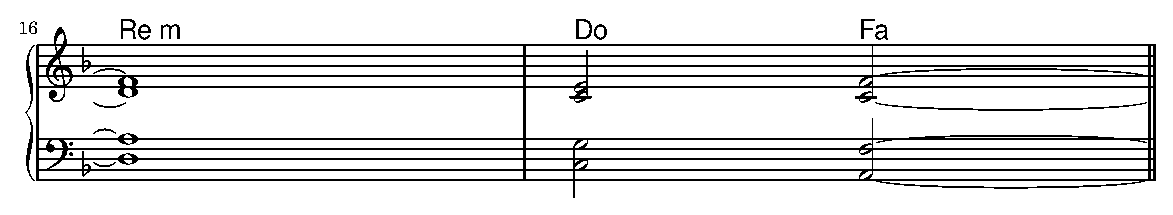
\includegraphics{f9/lily-e9938ef7-8}%
\ifx\betweenLilyPondSystem \undefined
  \linebreak
\else
  \expandafter\betweenLilyPondSystem{8}%
\fi

\includegraphics{f9/lily-e9938ef7-9}%
\ifx\betweenLilyPondSystem \undefined
  \linebreak
\else
  \expandafter\betweenLilyPondSystem{9}%
\fi

\includegraphics{f9/lily-e9938ef7-10}%
\ifx\betweenLilyPondSystem \undefined
  \linebreak
\else
  \expandafter\betweenLilyPondSystem{10}%
\fi
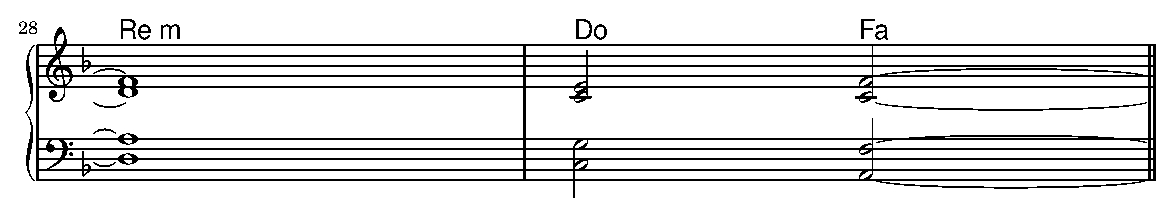
\includegraphics{f9/lily-e9938ef7-11}%
\ifx\betweenLilyPondSystem \undefined
  \linebreak
\else
  \expandafter\betweenLilyPondSystem{11}%
\fi

\includegraphics{f9/lily-e9938ef7-12}%
\ifx\betweenLilyPondSystem \undefined
  \linebreak
\else
  \expandafter\betweenLilyPondSystem{12}%
\fi

\includegraphics{f9/lily-e9938ef7-13}%
\ifx\betweenLilyPondSystem \undefined
  \linebreak
\else
  \expandafter\betweenLilyPondSystem{13}%
\fi

\includegraphics{f9/lily-e9938ef7-14}%
\ifx\betweenLilyPondSystem \undefined
  \linebreak
\else
  \expandafter\betweenLilyPondSystem{14}%
\fi

\includegraphics{f9/lily-e9938ef7-15}%
% eof
%
\ifx\postLilyPondExample \undefined
\else
  \expandafter\postLilyPondExample
\fi
}
    \clearpage

    {%
\parindent 0pt
\noindent
\ifx\preLilyPondExample \undefined
\else
  \expandafter\preLilyPondExample
\fi
\def\lilypondbook{}%

\includegraphics{67/lily-141e57bb-1}%
\ifx\betweenLilyPondSystem \undefined
  \linebreak
\else
  \expandafter\betweenLilyPondSystem{1}%
\fi

\includegraphics{67/lily-141e57bb-2}%
\ifx\betweenLilyPondSystem \undefined
  \linebreak
\else
  \expandafter\betweenLilyPondSystem{2}%
\fi

\includegraphics{67/lily-141e57bb-3}%
\ifx\betweenLilyPondSystem \undefined
  \linebreak
\else
  \expandafter\betweenLilyPondSystem{3}%
\fi

\includegraphics{67/lily-141e57bb-4}%
\ifx\betweenLilyPondSystem \undefined
  \linebreak
\else
  \expandafter\betweenLilyPondSystem{4}%
\fi

\includegraphics{67/lily-141e57bb-5}%
\ifx\betweenLilyPondSystem \undefined
  \linebreak
\else
  \expandafter\betweenLilyPondSystem{5}%
\fi

\includegraphics{67/lily-141e57bb-6}%
\ifx\betweenLilyPondSystem \undefined
  \linebreak
\else
  \expandafter\betweenLilyPondSystem{6}%
\fi

\includegraphics{67/lily-141e57bb-7}%
\ifx\betweenLilyPondSystem \undefined
  \linebreak
\else
  \expandafter\betweenLilyPondSystem{7}%
\fi

\includegraphics{67/lily-141e57bb-8}%
\ifx\betweenLilyPondSystem \undefined
  \linebreak
\else
  \expandafter\betweenLilyPondSystem{8}%
\fi

\includegraphics{67/lily-141e57bb-9}%
\ifx\betweenLilyPondSystem \undefined
  \linebreak
\else
  \expandafter\betweenLilyPondSystem{9}%
\fi

\includegraphics{67/lily-141e57bb-10}%
\ifx\betweenLilyPondSystem \undefined
  \linebreak
\else
  \expandafter\betweenLilyPondSystem{10}%
\fi

\includegraphics{67/lily-141e57bb-11}%
\ifx\betweenLilyPondSystem \undefined
  \linebreak
\else
  \expandafter\betweenLilyPondSystem{11}%
\fi

\includegraphics{67/lily-141e57bb-12}%
\ifx\betweenLilyPondSystem \undefined
  \linebreak
\else
  \expandafter\betweenLilyPondSystem{12}%
\fi

\includegraphics{67/lily-141e57bb-13}%
% eof
%
\ifx\postLilyPondExample \undefined
\else
  \expandafter\postLilyPondExample
\fi
}
    \clearpage

    {%
\parindent 0pt
\noindent
\ifx\preLilyPondExample \undefined
\else
  \expandafter\preLilyPondExample
\fi
\def\lilypondbook{}%

\includegraphics{ac/lily-3cf03fb4-1}%
\ifx\betweenLilyPondSystem \undefined
  \linebreak
\else
  \expandafter\betweenLilyPondSystem{1}%
\fi

\includegraphics{ac/lily-3cf03fb4-2}%
\ifx\betweenLilyPondSystem \undefined
  \linebreak
\else
  \expandafter\betweenLilyPondSystem{2}%
\fi

\includegraphics{ac/lily-3cf03fb4-3}%
\ifx\betweenLilyPondSystem \undefined
  \linebreak
\else
  \expandafter\betweenLilyPondSystem{3}%
\fi

\includegraphics{ac/lily-3cf03fb4-4}%
\ifx\betweenLilyPondSystem \undefined
  \linebreak
\else
  \expandafter\betweenLilyPondSystem{4}%
\fi

\includegraphics{ac/lily-3cf03fb4-5}%
\ifx\betweenLilyPondSystem \undefined
  \linebreak
\else
  \expandafter\betweenLilyPondSystem{5}%
\fi

\includegraphics{ac/lily-3cf03fb4-6}%
\ifx\betweenLilyPondSystem \undefined
  \linebreak
\else
  \expandafter\betweenLilyPondSystem{6}%
\fi

\includegraphics{ac/lily-3cf03fb4-7}%
\ifx\betweenLilyPondSystem \undefined
  \linebreak
\else
  \expandafter\betweenLilyPondSystem{7}%
\fi

\includegraphics{ac/lily-3cf03fb4-8}%
\ifx\betweenLilyPondSystem \undefined
  \linebreak
\else
  \expandafter\betweenLilyPondSystem{8}%
\fi

\includegraphics{ac/lily-3cf03fb4-9}%
\ifx\betweenLilyPondSystem \undefined
  \linebreak
\else
  \expandafter\betweenLilyPondSystem{9}%
\fi

\includegraphics{ac/lily-3cf03fb4-10}%
\ifx\betweenLilyPondSystem \undefined
  \linebreak
\else
  \expandafter\betweenLilyPondSystem{10}%
\fi

\includegraphics{ac/lily-3cf03fb4-11}%
\ifx\betweenLilyPondSystem \undefined
  \linebreak
\else
  \expandafter\betweenLilyPondSystem{11}%
\fi

\includegraphics{ac/lily-3cf03fb4-12}%
\ifx\betweenLilyPondSystem \undefined
  \linebreak
\else
  \expandafter\betweenLilyPondSystem{12}%
\fi

\includegraphics{ac/lily-3cf03fb4-13}%
% eof
%
\ifx\postLilyPondExample \undefined
\else
  \expandafter\postLilyPondExample
\fi
}
    \clearpage

    %% - Gloria in excelsis Deo - Melodia a modo del renacimiento
    \begin{center}
      \LARGE \textbf{Gloria a Dios en lo alto del cielo}
    \end{center}

    \Large El canto ``Gloria a Dios en lo alto del cielo'' es de melod\'ia alegre y r\'apida, tratando de mantener la forma sil\'abica de la versi\'on gregoriana. Contiene tambi\'en tres solos a forma de tono gregoriano para descanso del coro y acompa\~nar la din\'amica del texto en las suplicas al cordero. La invocaci\'on inicial tambien esta pensada para ser cantada por el celebrante o un miembro del coro.  Estos descansos tambi\'en sirven para que el canto en general no se sienta con prisa por terminarse.

    \noindent
    \LARGE Gloria a Dios en lo alto del cielo.\\
    Y en la tierra paz a los hombres que ama el Se\~nor. \\
    Te alabamos, te glorificamos, te damos gracias por tu gloria.

    \noindent
    Se\~nor Dios, Rey celestial, Dios Padre todopoderoso. \\
    Se\~nor, Hijo \'unico, Jesucristo.

    \noindent
    Se\~nor Dios, Cordero de Dios, Hijo del Padre, \\
    T\'u que quitas el pecado del mundo, ten piedad de nosotros.

    \noindent
    T\'u que quitas el pecado del mundo, atiende a nuestra s\'uplica. \\
    T\'u, que est\'as sentado a la derecha del Padre, ten piedad de nosotros.\\
    Porque s\'olo T\'u eres Santo, Se\~nor alt\'isimo Jesucristo. \\
    Con el Esp\'iritu Santo en la gloria.\\
    Am\'en.
    \clearpage

    {%
\parindent 0pt
\noindent
\ifx\preLilyPondExample \undefined
\else
  \expandafter\preLilyPondExample
\fi
\def\lilypondbook{}%

\includegraphics{99/lily-924018f8-1}%
\ifx\betweenLilyPondSystem \undefined
  \linebreak
\else
  \expandafter\betweenLilyPondSystem{1}%
\fi

\includegraphics{99/lily-924018f8-2}%
\ifx\betweenLilyPondSystem \undefined
  \linebreak
\else
  \expandafter\betweenLilyPondSystem{2}%
\fi

\includegraphics{99/lily-924018f8-3}%
\ifx\betweenLilyPondSystem \undefined
  \linebreak
\else
  \expandafter\betweenLilyPondSystem{3}%
\fi

\includegraphics{99/lily-924018f8-4}%
\ifx\betweenLilyPondSystem \undefined
  \linebreak
\else
  \expandafter\betweenLilyPondSystem{4}%
\fi

\includegraphics{99/lily-924018f8-5}%
\ifx\betweenLilyPondSystem \undefined
  \linebreak
\else
  \expandafter\betweenLilyPondSystem{5}%
\fi

\includegraphics{99/lily-924018f8-6}%
\ifx\betweenLilyPondSystem \undefined
  \linebreak
\else
  \expandafter\betweenLilyPondSystem{6}%
\fi

\includegraphics{99/lily-924018f8-7}%
\ifx\betweenLilyPondSystem \undefined
  \linebreak
\else
  \expandafter\betweenLilyPondSystem{7}%
\fi

\includegraphics{99/lily-924018f8-8}%
\ifx\betweenLilyPondSystem \undefined
  \linebreak
\else
  \expandafter\betweenLilyPondSystem{8}%
\fi
\includegraphics{99/lily-924018f8-9}%
\ifx\betweenLilyPondSystem \undefined
  \linebreak
\else
  \expandafter\betweenLilyPondSystem{9}%
\fi
\includegraphics{99/lily-924018f8-10}%
\ifx\betweenLilyPondSystem \undefined
  \linebreak
\else
  \expandafter\betweenLilyPondSystem{10}%
\fi
\includegraphics{99/lily-924018f8-11}%
\ifx\betweenLilyPondSystem \undefined
  \linebreak
\else
  \expandafter\betweenLilyPondSystem{11}%
\fi
\includegraphics{99/lily-924018f8-12}%
\ifx\betweenLilyPondSystem \undefined
  \linebreak
\else
  \expandafter\betweenLilyPondSystem{12}%
\fi
\includegraphics{99/lily-924018f8-13}%
\ifx\betweenLilyPondSystem \undefined
  \linebreak
\else
  \expandafter\betweenLilyPondSystem{13}%
\fi
\includegraphics{99/lily-924018f8-14}%
\ifx\betweenLilyPondSystem \undefined
  \linebreak
\else
  \expandafter\betweenLilyPondSystem{14}%
\fi
\includegraphics{99/lily-924018f8-15}%
\ifx\betweenLilyPondSystem \undefined
  \linebreak
\else
  \expandafter\betweenLilyPondSystem{15}%
\fi
\includegraphics{99/lily-924018f8-16}%
\ifx\betweenLilyPondSystem \undefined
  \linebreak
\else
  \expandafter\betweenLilyPondSystem{16}%
\fi
\includegraphics{99/lily-924018f8-17}%
\ifx\betweenLilyPondSystem \undefined
  \linebreak
\else
  \expandafter\betweenLilyPondSystem{17}%
\fi
\includegraphics{99/lily-924018f8-18}%
% eof
%
\ifx\postLilyPondExample \undefined
\else
  \expandafter\postLilyPondExample
\fi
}
    \clearpage

    {%
\parindent 0pt
\noindent
\ifx\preLilyPondExample \undefined
\else
  \expandafter\preLilyPondExample
\fi
\def\lilypondbook{}%
\includegraphics{da/lily-783406df-1}%
\ifx\betweenLilyPondSystem \undefined
  \linebreak
\else
  \expandafter\betweenLilyPondSystem{1}%
\fi
\includegraphics{da/lily-783406df-2}%
\ifx\betweenLilyPondSystem \undefined
  \linebreak
\else
  \expandafter\betweenLilyPondSystem{2}%
\fi
\includegraphics{da/lily-783406df-3}%
\ifx\betweenLilyPondSystem \undefined
  \linebreak
\else
  \expandafter\betweenLilyPondSystem{3}%
\fi
\includegraphics{da/lily-783406df-4}%
\ifx\betweenLilyPondSystem \undefined
  \linebreak
\else
  \expandafter\betweenLilyPondSystem{4}%
\fi
\includegraphics{da/lily-783406df-5}%
\ifx\betweenLilyPondSystem \undefined
  \linebreak
\else
  \expandafter\betweenLilyPondSystem{5}%
\fi
\includegraphics{da/lily-783406df-6}%
\ifx\betweenLilyPondSystem \undefined
  \linebreak
\else
  \expandafter\betweenLilyPondSystem{6}%
\fi
\includegraphics{da/lily-783406df-7}%
\ifx\betweenLilyPondSystem \undefined
  \linebreak
\else
  \expandafter\betweenLilyPondSystem{7}%
\fi
\includegraphics{da/lily-783406df-8}%
\ifx\betweenLilyPondSystem \undefined
  \linebreak
\else
  \expandafter\betweenLilyPondSystem{8}%
\fi
\includegraphics{da/lily-783406df-9}%
\ifx\betweenLilyPondSystem \undefined
  \linebreak
\else
  \expandafter\betweenLilyPondSystem{9}%
\fi
\includegraphics{da/lily-783406df-10}%
\ifx\betweenLilyPondSystem \undefined
  \linebreak
\else
  \expandafter\betweenLilyPondSystem{10}%
\fi
\includegraphics{da/lily-783406df-11}%
\ifx\betweenLilyPondSystem \undefined
  \linebreak
\else
  \expandafter\betweenLilyPondSystem{11}%
\fi
\includegraphics{da/lily-783406df-12}%
\ifx\betweenLilyPondSystem \undefined
  \linebreak
\else
  \expandafter\betweenLilyPondSystem{12}%
\fi
\includegraphics{da/lily-783406df-13}%
\ifx\betweenLilyPondSystem \undefined
  \linebreak
\else
  \expandafter\betweenLilyPondSystem{13}%
\fi
\includegraphics{da/lily-783406df-14}%
\ifx\betweenLilyPondSystem \undefined
  \linebreak
\else
  \expandafter\betweenLilyPondSystem{14}%
\fi
\includegraphics{da/lily-783406df-15}%
\ifx\betweenLilyPondSystem \undefined
  \linebreak
\else
  \expandafter\betweenLilyPondSystem{15}%
\fi
\includegraphics{da/lily-783406df-16}%
% eof
%
\ifx\postLilyPondExample \undefined
\else
  \expandafter\postLilyPondExample
\fi
}
    \clearpage

    {%
\parindent 0pt
\noindent
\ifx\preLilyPondExample \undefined
\else
  \expandafter\preLilyPondExample
\fi
\def\lilypondbook{}%
\includegraphics{cc/lily-65eae2d7-1}%
\ifx\betweenLilyPondSystem \undefined
  \linebreak
\else
  \expandafter\betweenLilyPondSystem{1}%
\fi
\includegraphics{cc/lily-65eae2d7-2}%
\ifx\betweenLilyPondSystem \undefined
  \linebreak
\else
  \expandafter\betweenLilyPondSystem{2}%
\fi
\includegraphics{cc/lily-65eae2d7-3}%
\ifx\betweenLilyPondSystem \undefined
  \linebreak
\else
  \expandafter\betweenLilyPondSystem{3}%
\fi
\includegraphics{cc/lily-65eae2d7-4}%
\ifx\betweenLilyPondSystem \undefined
  \linebreak
\else
  \expandafter\betweenLilyPondSystem{4}%
\fi
\includegraphics{cc/lily-65eae2d7-5}%
\ifx\betweenLilyPondSystem \undefined
  \linebreak
\else
  \expandafter\betweenLilyPondSystem{5}%
\fi
\includegraphics{cc/lily-65eae2d7-6}%
\ifx\betweenLilyPondSystem \undefined
  \linebreak
\else
  \expandafter\betweenLilyPondSystem{6}%
\fi
\includegraphics{cc/lily-65eae2d7-7}%
\ifx\betweenLilyPondSystem \undefined
  \linebreak
\else
  \expandafter\betweenLilyPondSystem{7}%
\fi
\includegraphics{cc/lily-65eae2d7-8}%
\ifx\betweenLilyPondSystem \undefined
  \linebreak
\else
  \expandafter\betweenLilyPondSystem{8}%
\fi
\includegraphics{cc/lily-65eae2d7-9}%
\ifx\betweenLilyPondSystem \undefined
  \linebreak
\else
  \expandafter\betweenLilyPondSystem{9}%
\fi
\includegraphics{cc/lily-65eae2d7-10}%
\ifx\betweenLilyPondSystem \undefined
  \linebreak
\else
  \expandafter\betweenLilyPondSystem{10}%
\fi
\includegraphics{cc/lily-65eae2d7-11}%
\ifx\betweenLilyPondSystem \undefined
  \linebreak
\else
  \expandafter\betweenLilyPondSystem{11}%
\fi
\includegraphics{cc/lily-65eae2d7-12}%
\ifx\betweenLilyPondSystem \undefined
  \linebreak
\else
  \expandafter\betweenLilyPondSystem{12}%
\fi
\includegraphics{cc/lily-65eae2d7-13}%
\ifx\betweenLilyPondSystem \undefined
  \linebreak
\else
  \expandafter\betweenLilyPondSystem{13}%
\fi
\includegraphics{cc/lily-65eae2d7-14}%
\ifx\betweenLilyPondSystem \undefined
  \linebreak
\else
  \expandafter\betweenLilyPondSystem{14}%
\fi
\includegraphics{cc/lily-65eae2d7-15}%
\ifx\betweenLilyPondSystem \undefined
  \linebreak
\else
  \expandafter\betweenLilyPondSystem{15}%
\fi
\includegraphics{cc/lily-65eae2d7-16}%
\ifx\betweenLilyPondSystem \undefined
  \linebreak
\else
  \expandafter\betweenLilyPondSystem{16}%
\fi
\includegraphics{cc/lily-65eae2d7-17}%
\ifx\betweenLilyPondSystem \undefined
  \linebreak
\else
  \expandafter\betweenLilyPondSystem{17}%
\fi
\includegraphics{cc/lily-65eae2d7-18}%
\ifx\betweenLilyPondSystem \undefined
  \linebreak
\else
  \expandafter\betweenLilyPondSystem{18}%
\fi
\includegraphics{cc/lily-65eae2d7-19}%
% eof
%
\ifx\postLilyPondExample \undefined
\else
  \expandafter\postLilyPondExample
\fi
}
    \clearpage

    %% - Credo in unum Deum - Melodia a modo del renacimiento
    \begin{center}
      \LARGE \textbf{Creo en Dios}
    \end{center}

    \Large El texto del canto ``Creo en Dios'' es tomado del Credo Apost\'olico, en las misas musicalizadas los m\'as usual es usar el texto del Credo Constantinopolitano pero debido a su extensi\'on nos pareci\'o no tan apropiado.\\
    Esta pieza tiene dos motivos, las invocaciones ``Creo en'' que son tres, \textit{Creo en Dios Padre}, \textit{Creo en Jesucristo} y \textit{Creo en el Esp\'iritu Santo}; las tres a modo de tono gregoriano seguida de una respuesta del coro con una melod\'ia muy solemne y majestuosa, con notas constantemente agudas y casi marcial, de nuevo estas partes fueron pensadas para que el celebrante las interprete y participe del canto, pero tambien pueden ser interpretadas por un miembro del coro.\\ La secci\'on central del Credo desde \textit{<<Padeci\'o bajo el poder...>>} hasta \textit{<<...a vivos y a muertos.>>} son dos solos, un solo de contralto cambiando a una melod\'ia y tiempo m\'as lento y triste pero a medida que llega la parte del texto que habla de la resurrecci\'on cambia al segundo solo, un solo de soprano con melod\'ia m\'as alegre y tiempo m\'as r\'apido desembocando en un d\'uo de contralto.

    \noindent
    \LARGE Creo en Dios.\\
    Padre todopoderoso creador del cielo y de la tierra.

    \noindent
    Creo en Jesucristo. \\
    Hijo \'unico, nuestro Se\~nor. Fue concebido por obra y gracia del Esp\'iritu Santo, nacio de Santa Mar\'ia Virgen.

    \noindent
    Padeci\'o bajo el poder de Poncio Pilato, fue crucificado, muerto y sepultado. Descendi\'o a los infiernos, al tercer d\'ia resucit\'o de entre los muertos, resucit\'o de entre los muertos. Subi\'o al cielo y est\'a sentado a la derecha de Dios Padre todopoderoso. Desde all\'i ha de venir a juzgar a vivos y a muertos.

    \noindent
    Creo en el Esp\'iritu Santo.\\
    La santa Iglesia cat\'olica, la comuni\'on de los santos, el perd\'on de los pecados, la resurrecci\'on de la carne y en la vida eterna.

    \noindent
    Am\'en.
    \clearpage

    {%
\parindent 0pt
\noindent
\ifx\preLilyPondExample \undefined
\else
  \expandafter\preLilyPondExample
\fi
\def\lilypondbook{}%
\includegraphics{a7/lily-613c5412-1}%
\ifx\betweenLilyPondSystem \undefined
  \linebreak
\else
  \expandafter\betweenLilyPondSystem{1}%
\fi
\includegraphics{a7/lily-613c5412-2}%
\ifx\betweenLilyPondSystem \undefined
  \linebreak
\else
  \expandafter\betweenLilyPondSystem{2}%
\fi
\includegraphics{a7/lily-613c5412-3}%
\ifx\betweenLilyPondSystem \undefined
  \linebreak
\else
  \expandafter\betweenLilyPondSystem{3}%
\fi
\includegraphics{a7/lily-613c5412-4}%
\ifx\betweenLilyPondSystem \undefined
  \linebreak
\else
  \expandafter\betweenLilyPondSystem{4}%
\fi
\includegraphics{a7/lily-613c5412-5}%
\ifx\betweenLilyPondSystem \undefined
  \linebreak
\else
  \expandafter\betweenLilyPondSystem{5}%
\fi
\includegraphics{a7/lily-613c5412-6}%
\ifx\betweenLilyPondSystem \undefined
  \linebreak
\else
  \expandafter\betweenLilyPondSystem{6}%
\fi
\includegraphics{a7/lily-613c5412-7}%
\ifx\betweenLilyPondSystem \undefined
  \linebreak
\else
  \expandafter\betweenLilyPondSystem{7}%
\fi
\includegraphics{a7/lily-613c5412-8}%
\ifx\betweenLilyPondSystem \undefined
  \linebreak
\else
  \expandafter\betweenLilyPondSystem{8}%
\fi
\includegraphics{a7/lily-613c5412-9}%
\ifx\betweenLilyPondSystem \undefined
  \linebreak
\else
  \expandafter\betweenLilyPondSystem{9}%
\fi
\includegraphics{a7/lily-613c5412-10}%
\ifx\betweenLilyPondSystem \undefined
  \linebreak
\else
  \expandafter\betweenLilyPondSystem{10}%
\fi
\includegraphics{a7/lily-613c5412-11}%
\ifx\betweenLilyPondSystem \undefined
  \linebreak
\else
  \expandafter\betweenLilyPondSystem{11}%
\fi
\includegraphics{a7/lily-613c5412-12}%
\ifx\betweenLilyPondSystem \undefined
  \linebreak
\else
  \expandafter\betweenLilyPondSystem{12}%
\fi
\includegraphics{a7/lily-613c5412-13}%
\ifx\betweenLilyPondSystem \undefined
  \linebreak
\else
  \expandafter\betweenLilyPondSystem{13}%
\fi
\includegraphics{a7/lily-613c5412-14}%
\ifx\betweenLilyPondSystem \undefined
  \linebreak
\else
  \expandafter\betweenLilyPondSystem{14}%
\fi
\includegraphics{a7/lily-613c5412-15}%
\ifx\betweenLilyPondSystem \undefined
  \linebreak
\else
  \expandafter\betweenLilyPondSystem{15}%
\fi
\includegraphics{a7/lily-613c5412-16}%
\ifx\betweenLilyPondSystem \undefined
  \linebreak
\else
  \expandafter\betweenLilyPondSystem{16}%
\fi
\includegraphics{a7/lily-613c5412-17}%
\ifx\betweenLilyPondSystem \undefined
  \linebreak
\else
  \expandafter\betweenLilyPondSystem{17}%
\fi
\includegraphics{a7/lily-613c5412-18}%
\ifx\betweenLilyPondSystem \undefined
  \linebreak
\else
  \expandafter\betweenLilyPondSystem{18}%
\fi
\includegraphics{a7/lily-613c5412-19}%
\ifx\betweenLilyPondSystem \undefined
  \linebreak
\else
  \expandafter\betweenLilyPondSystem{19}%
\fi
\includegraphics{a7/lily-613c5412-20}%
\ifx\betweenLilyPondSystem \undefined
  \linebreak
\else
  \expandafter\betweenLilyPondSystem{20}%
\fi
\includegraphics{a7/lily-613c5412-21}%
\ifx\betweenLilyPondSystem \undefined
  \linebreak
\else
  \expandafter\betweenLilyPondSystem{21}%
\fi
\includegraphics{a7/lily-613c5412-22}%
\ifx\betweenLilyPondSystem \undefined
  \linebreak
\else
  \expandafter\betweenLilyPondSystem{22}%
\fi
\includegraphics{a7/lily-613c5412-23}%
\ifx\betweenLilyPondSystem \undefined
  \linebreak
\else
  \expandafter\betweenLilyPondSystem{23}%
\fi
\includegraphics{a7/lily-613c5412-24}%
% eof
%
\ifx\postLilyPondExample \undefined
\else
  \expandafter\postLilyPondExample
\fi
}
    \clearpage

    {%
\parindent 0pt
\noindent
\ifx\preLilyPondExample \undefined
\else
  \expandafter\preLilyPondExample
\fi
\def\lilypondbook{}%
\includegraphics{88/lily-74af5495-1}%
\ifx\betweenLilyPondSystem \undefined
  \linebreak
\else
  \expandafter\betweenLilyPondSystem{1}%
\fi
\includegraphics{88/lily-74af5495-2}%
\ifx\betweenLilyPondSystem \undefined
  \linebreak
\else
  \expandafter\betweenLilyPondSystem{2}%
\fi
\includegraphics{88/lily-74af5495-3}%
\ifx\betweenLilyPondSystem \undefined
  \linebreak
\else
  \expandafter\betweenLilyPondSystem{3}%
\fi
\includegraphics{88/lily-74af5495-4}%
\ifx\betweenLilyPondSystem \undefined
  \linebreak
\else
  \expandafter\betweenLilyPondSystem{4}%
\fi
\includegraphics{88/lily-74af5495-5}%
\ifx\betweenLilyPondSystem \undefined
  \linebreak
\else
  \expandafter\betweenLilyPondSystem{5}%
\fi
\includegraphics{88/lily-74af5495-6}%
\ifx\betweenLilyPondSystem \undefined
  \linebreak
\else
  \expandafter\betweenLilyPondSystem{6}%
\fi
\includegraphics{88/lily-74af5495-7}%
\ifx\betweenLilyPondSystem \undefined
  \linebreak
\else
  \expandafter\betweenLilyPondSystem{7}%
\fi
\includegraphics{88/lily-74af5495-8}%
\ifx\betweenLilyPondSystem \undefined
  \linebreak
\else
  \expandafter\betweenLilyPondSystem{8}%
\fi
\includegraphics{88/lily-74af5495-9}%
\ifx\betweenLilyPondSystem \undefined
  \linebreak
\else
  \expandafter\betweenLilyPondSystem{9}%
\fi
\includegraphics{88/lily-74af5495-10}%
\ifx\betweenLilyPondSystem \undefined
  \linebreak
\else
  \expandafter\betweenLilyPondSystem{10}%
\fi
\includegraphics{88/lily-74af5495-11}%
\ifx\betweenLilyPondSystem \undefined
  \linebreak
\else
  \expandafter\betweenLilyPondSystem{11}%
\fi
\includegraphics{88/lily-74af5495-12}%
\ifx\betweenLilyPondSystem \undefined
  \linebreak
\else
  \expandafter\betweenLilyPondSystem{12}%
\fi
\includegraphics{88/lily-74af5495-13}%
\ifx\betweenLilyPondSystem \undefined
  \linebreak
\else
  \expandafter\betweenLilyPondSystem{13}%
\fi
\includegraphics{88/lily-74af5495-14}%
\ifx\betweenLilyPondSystem \undefined
  \linebreak
\else
  \expandafter\betweenLilyPondSystem{14}%
\fi
\includegraphics{88/lily-74af5495-15}%
\ifx\betweenLilyPondSystem \undefined
  \linebreak
\else
  \expandafter\betweenLilyPondSystem{15}%
\fi
\includegraphics{88/lily-74af5495-16}%
\ifx\betweenLilyPondSystem \undefined
  \linebreak
\else
  \expandafter\betweenLilyPondSystem{16}%
\fi
\includegraphics{88/lily-74af5495-17}%
\ifx\betweenLilyPondSystem \undefined
  \linebreak
\else
  \expandafter\betweenLilyPondSystem{17}%
\fi
\includegraphics{88/lily-74af5495-18}%
\ifx\betweenLilyPondSystem \undefined
  \linebreak
\else
  \expandafter\betweenLilyPondSystem{18}%
\fi
\includegraphics{88/lily-74af5495-19}%
\ifx\betweenLilyPondSystem \undefined
  \linebreak
\else
  \expandafter\betweenLilyPondSystem{19}%
\fi
\includegraphics{88/lily-74af5495-20}%
\ifx\betweenLilyPondSystem \undefined
  \linebreak
\else
  \expandafter\betweenLilyPondSystem{20}%
\fi
\includegraphics{88/lily-74af5495-21}%
\ifx\betweenLilyPondSystem \undefined
  \linebreak
\else
  \expandafter\betweenLilyPondSystem{21}%
\fi
\includegraphics{88/lily-74af5495-22}%
\ifx\betweenLilyPondSystem \undefined
  \linebreak
\else
  \expandafter\betweenLilyPondSystem{22}%
\fi
\includegraphics{88/lily-74af5495-23}%
\ifx\betweenLilyPondSystem \undefined
  \linebreak
\else
  \expandafter\betweenLilyPondSystem{23}%
\fi
\includegraphics{88/lily-74af5495-24}%
% eof
%
\ifx\postLilyPondExample \undefined
\else
  \expandafter\postLilyPondExample
\fi
}
    \clearpage

    {%
\parindent 0pt
\noindent
\ifx\preLilyPondExample \undefined
\else
  \expandafter\preLilyPondExample
\fi
\def\lilypondbook{}%
\includegraphics{c6/lily-b8525778-1}%
\ifx\betweenLilyPondSystem \undefined
  \linebreak
\else
  \expandafter\betweenLilyPondSystem{1}%
\fi
\includegraphics{c6/lily-b8525778-2}%
\ifx\betweenLilyPondSystem \undefined
  \linebreak
\else
  \expandafter\betweenLilyPondSystem{2}%
\fi
\includegraphics{c6/lily-b8525778-3}%
\ifx\betweenLilyPondSystem \undefined
  \linebreak
\else
  \expandafter\betweenLilyPondSystem{3}%
\fi
\includegraphics{c6/lily-b8525778-4}%
\ifx\betweenLilyPondSystem \undefined
  \linebreak
\else
  \expandafter\betweenLilyPondSystem{4}%
\fi
\includegraphics{c6/lily-b8525778-5}%
\ifx\betweenLilyPondSystem \undefined
  \linebreak
\else
  \expandafter\betweenLilyPondSystem{5}%
\fi
\includegraphics{c6/lily-b8525778-6}%
\ifx\betweenLilyPondSystem \undefined
  \linebreak
\else
  \expandafter\betweenLilyPondSystem{6}%
\fi
\includegraphics{c6/lily-b8525778-7}%
\ifx\betweenLilyPondSystem \undefined
  \linebreak
\else
  \expandafter\betweenLilyPondSystem{7}%
\fi
\includegraphics{c6/lily-b8525778-8}%
\ifx\betweenLilyPondSystem \undefined
  \linebreak
\else
  \expandafter\betweenLilyPondSystem{8}%
\fi
\includegraphics{c6/lily-b8525778-9}%
\ifx\betweenLilyPondSystem \undefined
  \linebreak
\else
  \expandafter\betweenLilyPondSystem{9}%
\fi
\includegraphics{c6/lily-b8525778-10}%
\ifx\betweenLilyPondSystem \undefined
  \linebreak
\else
  \expandafter\betweenLilyPondSystem{10}%
\fi
\includegraphics{c6/lily-b8525778-11}%
\ifx\betweenLilyPondSystem \undefined
  \linebreak
\else
  \expandafter\betweenLilyPondSystem{11}%
\fi
\includegraphics{c6/lily-b8525778-12}%
\ifx\betweenLilyPondSystem \undefined
  \linebreak
\else
  \expandafter\betweenLilyPondSystem{12}%
\fi
\includegraphics{c6/lily-b8525778-13}%
\ifx\betweenLilyPondSystem \undefined
  \linebreak
\else
  \expandafter\betweenLilyPondSystem{13}%
\fi
\includegraphics{c6/lily-b8525778-14}%
\ifx\betweenLilyPondSystem \undefined
  \linebreak
\else
  \expandafter\betweenLilyPondSystem{14}%
\fi
\includegraphics{c6/lily-b8525778-15}%
\ifx\betweenLilyPondSystem \undefined
  \linebreak
\else
  \expandafter\betweenLilyPondSystem{15}%
\fi
\includegraphics{c6/lily-b8525778-16}%
\ifx\betweenLilyPondSystem \undefined
  \linebreak
\else
  \expandafter\betweenLilyPondSystem{16}%
\fi
\includegraphics{c6/lily-b8525778-17}%
\ifx\betweenLilyPondSystem \undefined
  \linebreak
\else
  \expandafter\betweenLilyPondSystem{17}%
\fi
\includegraphics{c6/lily-b8525778-18}%
\ifx\betweenLilyPondSystem \undefined
  \linebreak
\else
  \expandafter\betweenLilyPondSystem{18}%
\fi
\includegraphics{c6/lily-b8525778-19}%
\ifx\betweenLilyPondSystem \undefined
  \linebreak
\else
  \expandafter\betweenLilyPondSystem{19}%
\fi
\includegraphics{c6/lily-b8525778-20}%
\ifx\betweenLilyPondSystem \undefined
  \linebreak
\else
  \expandafter\betweenLilyPondSystem{20}%
\fi
\includegraphics{c6/lily-b8525778-21}%
\ifx\betweenLilyPondSystem \undefined
  \linebreak
\else
  \expandafter\betweenLilyPondSystem{21}%
\fi
\includegraphics{c6/lily-b8525778-22}%
\ifx\betweenLilyPondSystem \undefined
  \linebreak
\else
  \expandafter\betweenLilyPondSystem{22}%
\fi
\includegraphics{c6/lily-b8525778-23}%
\ifx\betweenLilyPondSystem \undefined
  \linebreak
\else
  \expandafter\betweenLilyPondSystem{23}%
\fi
\includegraphics{c6/lily-b8525778-24}%
\ifx\betweenLilyPondSystem \undefined
  \linebreak
\else
  \expandafter\betweenLilyPondSystem{24}%
\fi
\includegraphics{c6/lily-b8525778-25}%
% eof
%
\ifx\postLilyPondExample \undefined
\else
  \expandafter\postLilyPondExample
\fi
}
    \clearpage

    %% - Sanctus - Melodia a modo del renacimiento
    \begin{center}
      \LARGE \textbf{Santo}
    \end{center}

    \Large El canto ``Santo'' sigue la misma linea del canto ``Gloria a Dios en lo alto del cielo'' en lo alegre y en la velocidad, sin embargo este canto no tiene reposo excepto por la invocaci\'on inicial; tambien pensada para ser interpreta por el celebrante o un miembro del coro. Su melod\'ia cantada por todo el coro sin solos, esta dispuesta en dos parte, la primera parte desde el trisagio \textit{<<Santo, santo, santo...>>} hasta \textit{<<...llenos de tu gloria>>} y \textit{<<...nombre del Se\~nor>>} y la segunda el Hossana que es al doble de la velocidad del resto del canto asemejando a las piezas separadas que era antiguamente por la diferencia de tiempo.

    \noindent
    \LARGE Santo

    \noindent
    \LARGE Santo, santo, santo. \\
    Los cielos y la tierra est\'an llenos de tu gloria.\\
    Hosana, hosana, en el cielo.\\
    Bendito el que viene en el nombre del Se\~nor. \\
    Hosana, hosana, en el cielo.
    \clearpage

    {%
\parindent 0pt
\noindent
\ifx\preLilyPondExample \undefined
\else
  \expandafter\preLilyPondExample
\fi
\def\lilypondbook{}%
\includegraphics{25/lily-82b181f0-1}%
\ifx\betweenLilyPondSystem \undefined
  \linebreak
\else
  \expandafter\betweenLilyPondSystem{1}%
\fi
\includegraphics{25/lily-82b181f0-2}%
\ifx\betweenLilyPondSystem \undefined
  \linebreak
\else
  \expandafter\betweenLilyPondSystem{2}%
\fi
\includegraphics{25/lily-82b181f0-3}%
\ifx\betweenLilyPondSystem \undefined
  \linebreak
\else
  \expandafter\betweenLilyPondSystem{3}%
\fi
\includegraphics{25/lily-82b181f0-4}%
\ifx\betweenLilyPondSystem \undefined
  \linebreak
\else
  \expandafter\betweenLilyPondSystem{4}%
\fi
\includegraphics{25/lily-82b181f0-5}%
\ifx\betweenLilyPondSystem \undefined
  \linebreak
\else
  \expandafter\betweenLilyPondSystem{5}%
\fi
\includegraphics{25/lily-82b181f0-6}%
\ifx\betweenLilyPondSystem \undefined
  \linebreak
\else
  \expandafter\betweenLilyPondSystem{6}%
\fi
\includegraphics{25/lily-82b181f0-7}%
\ifx\betweenLilyPondSystem \undefined
  \linebreak
\else
  \expandafter\betweenLilyPondSystem{7}%
\fi
\includegraphics{25/lily-82b181f0-8}%
\ifx\betweenLilyPondSystem \undefined
  \linebreak
\else
  \expandafter\betweenLilyPondSystem{8}%
\fi
\includegraphics{25/lily-82b181f0-9}%
\ifx\betweenLilyPondSystem \undefined
  \linebreak
\else
  \expandafter\betweenLilyPondSystem{9}%
\fi
\includegraphics{25/lily-82b181f0-10}%
\ifx\betweenLilyPondSystem \undefined
  \linebreak
\else
  \expandafter\betweenLilyPondSystem{10}%
\fi
\includegraphics{25/lily-82b181f0-11}%
\ifx\betweenLilyPondSystem \undefined
  \linebreak
\else
  \expandafter\betweenLilyPondSystem{11}%
\fi
\includegraphics{25/lily-82b181f0-12}%
\ifx\betweenLilyPondSystem \undefined
  \linebreak
\else
  \expandafter\betweenLilyPondSystem{12}%
\fi
\includegraphics{25/lily-82b181f0-13}%
\ifx\betweenLilyPondSystem \undefined
  \linebreak
\else
  \expandafter\betweenLilyPondSystem{13}%
\fi
\includegraphics{25/lily-82b181f0-14}%
\ifx\betweenLilyPondSystem \undefined
  \linebreak
\else
  \expandafter\betweenLilyPondSystem{14}%
\fi
\includegraphics{25/lily-82b181f0-15}%
\ifx\betweenLilyPondSystem \undefined
  \linebreak
\else
  \expandafter\betweenLilyPondSystem{15}%
\fi
\includegraphics{25/lily-82b181f0-16}%
% eof
%
\ifx\postLilyPondExample \undefined
\else
  \expandafter\postLilyPondExample
\fi
}
    \clearpage

    {%
\parindent 0pt
\noindent
\ifx\preLilyPondExample \undefined
\else
  \expandafter\preLilyPondExample
\fi
\def\lilypondbook{}%
\includegraphics{00/lily-ee0cfb43-1}%
\ifx\betweenLilyPondSystem \undefined
  \linebreak
\else
  \expandafter\betweenLilyPondSystem{1}%
\fi
\includegraphics{00/lily-ee0cfb43-2}%
\ifx\betweenLilyPondSystem \undefined
  \linebreak
\else
  \expandafter\betweenLilyPondSystem{2}%
\fi
\includegraphics{00/lily-ee0cfb43-3}%
\ifx\betweenLilyPondSystem \undefined
  \linebreak
\else
  \expandafter\betweenLilyPondSystem{3}%
\fi
\includegraphics{00/lily-ee0cfb43-4}%
\ifx\betweenLilyPondSystem \undefined
  \linebreak
\else
  \expandafter\betweenLilyPondSystem{4}%
\fi
\includegraphics{00/lily-ee0cfb43-5}%
\ifx\betweenLilyPondSystem \undefined
  \linebreak
\else
  \expandafter\betweenLilyPondSystem{5}%
\fi
\includegraphics{00/lily-ee0cfb43-6}%
\ifx\betweenLilyPondSystem \undefined
  \linebreak
\else
  \expandafter\betweenLilyPondSystem{6}%
\fi
\includegraphics{00/lily-ee0cfb43-7}%
\ifx\betweenLilyPondSystem \undefined
  \linebreak
\else
  \expandafter\betweenLilyPondSystem{7}%
\fi
\includegraphics{00/lily-ee0cfb43-8}%
\ifx\betweenLilyPondSystem \undefined
  \linebreak
\else
  \expandafter\betweenLilyPondSystem{8}%
\fi
\includegraphics{00/lily-ee0cfb43-9}%
\ifx\betweenLilyPondSystem \undefined
  \linebreak
\else
  \expandafter\betweenLilyPondSystem{9}%
\fi
\includegraphics{00/lily-ee0cfb43-10}%
\ifx\betweenLilyPondSystem \undefined
  \linebreak
\else
  \expandafter\betweenLilyPondSystem{10}%
\fi
\includegraphics{00/lily-ee0cfb43-11}%
\ifx\betweenLilyPondSystem \undefined
  \linebreak
\else
  \expandafter\betweenLilyPondSystem{11}%
\fi
\includegraphics{00/lily-ee0cfb43-12}%
\ifx\betweenLilyPondSystem \undefined
  \linebreak
\else
  \expandafter\betweenLilyPondSystem{12}%
\fi
\includegraphics{00/lily-ee0cfb43-13}%
\ifx\betweenLilyPondSystem \undefined
  \linebreak
\else
  \expandafter\betweenLilyPondSystem{13}%
\fi
\includegraphics{00/lily-ee0cfb43-14}%
\ifx\betweenLilyPondSystem \undefined
  \linebreak
\else
  \expandafter\betweenLilyPondSystem{14}%
\fi
\includegraphics{00/lily-ee0cfb43-15}%
% eof
%
\ifx\postLilyPondExample \undefined
\else
  \expandafter\postLilyPondExample
\fi
}
    \clearpage

    {%
\parindent 0pt
\noindent
\ifx\preLilyPondExample \undefined
\else
  \expandafter\preLilyPondExample
\fi
\def\lilypondbook{}%
\includegraphics{bb/lily-e47debc8-1}%
\ifx\betweenLilyPondSystem \undefined
  \linebreak
\else
  \expandafter\betweenLilyPondSystem{1}%
\fi
\includegraphics{bb/lily-e47debc8-2}%
\ifx\betweenLilyPondSystem \undefined
  \linebreak
\else
  \expandafter\betweenLilyPondSystem{2}%
\fi
\includegraphics{bb/lily-e47debc8-3}%
\ifx\betweenLilyPondSystem \undefined
  \linebreak
\else
  \expandafter\betweenLilyPondSystem{3}%
\fi
\includegraphics{bb/lily-e47debc8-4}%
\ifx\betweenLilyPondSystem \undefined
  \linebreak
\else
  \expandafter\betweenLilyPondSystem{4}%
\fi
\includegraphics{bb/lily-e47debc8-5}%
\ifx\betweenLilyPondSystem \undefined
  \linebreak
\else
  \expandafter\betweenLilyPondSystem{5}%
\fi
\includegraphics{bb/lily-e47debc8-6}%
\ifx\betweenLilyPondSystem \undefined
  \linebreak
\else
  \expandafter\betweenLilyPondSystem{6}%
\fi
\includegraphics{bb/lily-e47debc8-7}%
\ifx\betweenLilyPondSystem \undefined
  \linebreak
\else
  \expandafter\betweenLilyPondSystem{7}%
\fi
\includegraphics{bb/lily-e47debc8-8}%
\ifx\betweenLilyPondSystem \undefined
  \linebreak
\else
  \expandafter\betweenLilyPondSystem{8}%
\fi
\includegraphics{bb/lily-e47debc8-9}%
\ifx\betweenLilyPondSystem \undefined
  \linebreak
\else
  \expandafter\betweenLilyPondSystem{9}%
\fi
\includegraphics{bb/lily-e47debc8-10}%
\ifx\betweenLilyPondSystem \undefined
  \linebreak
\else
  \expandafter\betweenLilyPondSystem{10}%
\fi
\includegraphics{bb/lily-e47debc8-11}%
\ifx\betweenLilyPondSystem \undefined
  \linebreak
\else
  \expandafter\betweenLilyPondSystem{11}%
\fi
\includegraphics{bb/lily-e47debc8-12}%
\ifx\betweenLilyPondSystem \undefined
  \linebreak
\else
  \expandafter\betweenLilyPondSystem{12}%
\fi
\includegraphics{bb/lily-e47debc8-13}%
\ifx\betweenLilyPondSystem \undefined
  \linebreak
\else
  \expandafter\betweenLilyPondSystem{13}%
\fi
\includegraphics{bb/lily-e47debc8-14}%
\ifx\betweenLilyPondSystem \undefined
  \linebreak
\else
  \expandafter\betweenLilyPondSystem{14}%
\fi
\includegraphics{bb/lily-e47debc8-15}%
% eof
%
\ifx\postLilyPondExample \undefined
\else
  \expandafter\postLilyPondExample
\fi
}
    \clearpage

    %% - Agnus Dei - Melodia a modo del renacimiento
    \begin{center}
      \LARGE \textbf{Cordero de Dios}
    \end{center}

    \Large El canto ``Cordero de Dios'' tiene una melod\'ia m\'as solemne e invita a la adoraci\'on y reflexi\'on. El canto posee tres invocaciones a modo de tono gregoriano, tambien par ser interpretadas por el celebrante, al inicio de la letan\'ia a la que se suma el coro. Las respuestas \textit{<<Ten piedad de nosotros>>} y \textit{<<Danos la paz>>}, tienen una melod\'ia un poco m\'as simple para que la asamblea pueda responder junto con el coro.

    \noindent
    \LARGE Cordero de Dios.\\
    Que quitas el pecado del mundo. Ten piedad de nosotros.

    \noindent
    \LARGE Cordero de Dios.\\
    Que quitas el pecado del mundo. Ten piedad de nosotros.

    \noindent
    \LARGE Cordero de Dios.\\
    Que quitas el pecado del mundo. Danos la paz.
    \clearpage

    {%
\parindent 0pt
\noindent
\ifx\preLilyPondExample \undefined
\else
  \expandafter\preLilyPondExample
\fi
\def\lilypondbook{}%
\includegraphics{9c/lily-6f50c4a7-1}%
\ifx\betweenLilyPondSystem \undefined
  \linebreak
\else
  \expandafter\betweenLilyPondSystem{1}%
\fi
\includegraphics{9c/lily-6f50c4a7-2}%
\ifx\betweenLilyPondSystem \undefined
  \linebreak
\else
  \expandafter\betweenLilyPondSystem{2}%
\fi
\includegraphics{9c/lily-6f50c4a7-3}%
\ifx\betweenLilyPondSystem \undefined
  \linebreak
\else
  \expandafter\betweenLilyPondSystem{3}%
\fi
\includegraphics{9c/lily-6f50c4a7-4}%
\ifx\betweenLilyPondSystem \undefined
  \linebreak
\else
  \expandafter\betweenLilyPondSystem{4}%
\fi
\includegraphics{9c/lily-6f50c4a7-5}%
\ifx\betweenLilyPondSystem \undefined
  \linebreak
\else
  \expandafter\betweenLilyPondSystem{5}%
\fi
\includegraphics{9c/lily-6f50c4a7-6}%
\ifx\betweenLilyPondSystem \undefined
  \linebreak
\else
  \expandafter\betweenLilyPondSystem{6}%
\fi
\includegraphics{9c/lily-6f50c4a7-7}%
\ifx\betweenLilyPondSystem \undefined
  \linebreak
\else
  \expandafter\betweenLilyPondSystem{7}%
\fi
\includegraphics{9c/lily-6f50c4a7-8}%
\ifx\betweenLilyPondSystem \undefined
  \linebreak
\else
  \expandafter\betweenLilyPondSystem{8}%
\fi
\includegraphics{9c/lily-6f50c4a7-9}%
\ifx\betweenLilyPondSystem \undefined
  \linebreak
\else
  \expandafter\betweenLilyPondSystem{9}%
\fi
\includegraphics{9c/lily-6f50c4a7-10}%
\ifx\betweenLilyPondSystem \undefined
  \linebreak
\else
  \expandafter\betweenLilyPondSystem{10}%
\fi
\includegraphics{9c/lily-6f50c4a7-11}%
\ifx\betweenLilyPondSystem \undefined
  \linebreak
\else
  \expandafter\betweenLilyPondSystem{11}%
\fi
\includegraphics{9c/lily-6f50c4a7-12}%
\ifx\betweenLilyPondSystem \undefined
  \linebreak
\else
  \expandafter\betweenLilyPondSystem{12}%
\fi
\includegraphics{9c/lily-6f50c4a7-13}%
\ifx\betweenLilyPondSystem \undefined
  \linebreak
\else
  \expandafter\betweenLilyPondSystem{13}%
\fi
\includegraphics{9c/lily-6f50c4a7-14}%
% eof
%
\ifx\postLilyPondExample \undefined
\else
  \expandafter\postLilyPondExample
\fi
}
    \clearpage

    {%
\parindent 0pt
\noindent
\ifx\preLilyPondExample \undefined
\else
  \expandafter\preLilyPondExample
\fi
\def\lilypondbook{}%
\includegraphics{33/lily-a7cdee07-1}%
\ifx\betweenLilyPondSystem \undefined
  \linebreak
\else
  \expandafter\betweenLilyPondSystem{1}%
\fi
\includegraphics{33/lily-a7cdee07-2}%
\ifx\betweenLilyPondSystem \undefined
  \linebreak
\else
  \expandafter\betweenLilyPondSystem{2}%
\fi
\includegraphics{33/lily-a7cdee07-3}%
\ifx\betweenLilyPondSystem \undefined
  \linebreak
\else
  \expandafter\betweenLilyPondSystem{3}%
\fi
\includegraphics{33/lily-a7cdee07-4}%
\ifx\betweenLilyPondSystem \undefined
  \linebreak
\else
  \expandafter\betweenLilyPondSystem{4}%
\fi
\includegraphics{33/lily-a7cdee07-5}%
\ifx\betweenLilyPondSystem \undefined
  \linebreak
\else
  \expandafter\betweenLilyPondSystem{5}%
\fi
\includegraphics{33/lily-a7cdee07-6}%
\ifx\betweenLilyPondSystem \undefined
  \linebreak
\else
  \expandafter\betweenLilyPondSystem{6}%
\fi
\includegraphics{33/lily-a7cdee07-7}%
\ifx\betweenLilyPondSystem \undefined
  \linebreak
\else
  \expandafter\betweenLilyPondSystem{7}%
\fi
\includegraphics{33/lily-a7cdee07-8}%
\ifx\betweenLilyPondSystem \undefined
  \linebreak
\else
  \expandafter\betweenLilyPondSystem{8}%
\fi
\includegraphics{33/lily-a7cdee07-9}%
\ifx\betweenLilyPondSystem \undefined
  \linebreak
\else
  \expandafter\betweenLilyPondSystem{9}%
\fi
\includegraphics{33/lily-a7cdee07-10}%
\ifx\betweenLilyPondSystem \undefined
  \linebreak
\else
  \expandafter\betweenLilyPondSystem{10}%
\fi
\includegraphics{33/lily-a7cdee07-11}%
\ifx\betweenLilyPondSystem \undefined
  \linebreak
\else
  \expandafter\betweenLilyPondSystem{11}%
\fi
\includegraphics{33/lily-a7cdee07-12}%
\ifx\betweenLilyPondSystem \undefined
  \linebreak
\else
  \expandafter\betweenLilyPondSystem{12}%
\fi
\includegraphics{33/lily-a7cdee07-13}%
\ifx\betweenLilyPondSystem \undefined
  \linebreak
\else
  \expandafter\betweenLilyPondSystem{13}%
\fi
\includegraphics{33/lily-a7cdee07-14}%
\ifx\betweenLilyPondSystem \undefined
  \linebreak
\else
  \expandafter\betweenLilyPondSystem{14}%
\fi
\includegraphics{33/lily-a7cdee07-15}%
\ifx\betweenLilyPondSystem \undefined
  \linebreak
\else
  \expandafter\betweenLilyPondSystem{15}%
\fi
\includegraphics{33/lily-a7cdee07-16}%
% eof
%
\ifx\postLilyPondExample \undefined
\else
  \expandafter\postLilyPondExample
\fi
}
    \clearpage

    {%
\parindent 0pt
\noindent
\ifx\preLilyPondExample \undefined
\else
  \expandafter\preLilyPondExample
\fi
\def\lilypondbook{}%
\includegraphics{94/lily-bc6a4ac0-1}%
\ifx\betweenLilyPondSystem \undefined
  \linebreak
\else
  \expandafter\betweenLilyPondSystem{1}%
\fi
\includegraphics{94/lily-bc6a4ac0-2}%
\ifx\betweenLilyPondSystem \undefined
  \linebreak
\else
  \expandafter\betweenLilyPondSystem{2}%
\fi
\includegraphics{94/lily-bc6a4ac0-3}%
\ifx\betweenLilyPondSystem \undefined
  \linebreak
\else
  \expandafter\betweenLilyPondSystem{3}%
\fi
\includegraphics{94/lily-bc6a4ac0-4}%
\ifx\betweenLilyPondSystem \undefined
  \linebreak
\else
  \expandafter\betweenLilyPondSystem{4}%
\fi
\includegraphics{94/lily-bc6a4ac0-5}%
\ifx\betweenLilyPondSystem \undefined
  \linebreak
\else
  \expandafter\betweenLilyPondSystem{5}%
\fi
\includegraphics{94/lily-bc6a4ac0-6}%
\ifx\betweenLilyPondSystem \undefined
  \linebreak
\else
  \expandafter\betweenLilyPondSystem{6}%
\fi
\includegraphics{94/lily-bc6a4ac0-7}%
\ifx\betweenLilyPondSystem \undefined
  \linebreak
\else
  \expandafter\betweenLilyPondSystem{7}%
\fi
\includegraphics{94/lily-bc6a4ac0-8}%
\ifx\betweenLilyPondSystem \undefined
  \linebreak
\else
  \expandafter\betweenLilyPondSystem{8}%
\fi
\includegraphics{94/lily-bc6a4ac0-9}%
\ifx\betweenLilyPondSystem \undefined
  \linebreak
\else
  \expandafter\betweenLilyPondSystem{9}%
\fi
\includegraphics{94/lily-bc6a4ac0-10}%
\ifx\betweenLilyPondSystem \undefined
  \linebreak
\else
  \expandafter\betweenLilyPondSystem{10}%
\fi
\includegraphics{94/lily-bc6a4ac0-11}%
\ifx\betweenLilyPondSystem \undefined
  \linebreak
\else
  \expandafter\betweenLilyPondSystem{11}%
\fi
\includegraphics{94/lily-bc6a4ac0-12}%
\ifx\betweenLilyPondSystem \undefined
  \linebreak
\else
  \expandafter\betweenLilyPondSystem{12}%
\fi
\includegraphics{94/lily-bc6a4ac0-13}%
\ifx\betweenLilyPondSystem \undefined
  \linebreak
\else
  \expandafter\betweenLilyPondSystem{13}%
\fi
\includegraphics{94/lily-bc6a4ac0-14}%
\ifx\betweenLilyPondSystem \undefined
  \linebreak
\else
  \expandafter\betweenLilyPondSystem{14}%
\fi
\includegraphics{94/lily-bc6a4ac0-15}%
\ifx\betweenLilyPondSystem \undefined
  \linebreak
\else
  \expandafter\betweenLilyPondSystem{15}%
\fi
\includegraphics{94/lily-bc6a4ac0-16}%
% eof
%
\ifx\postLilyPondExample \undefined
\else
  \expandafter\postLilyPondExample
\fi
}
    \clearpage

    %% - Propio
    \begin{center}
      \vspace*{8cm}
      \textbf{\Huge Propio de la Misa}\\
      \textit{ \Large Solemnidad Cristo Rey del Universo}
    \end{center}
    \clearpage

    %% - Introito - Melodia a inspiracion de Mnsr. Marco Frisina
    \begin{center}
      \LARGE \textbf{Canto de Entrada}
    \end{center}

    \Large El texto del canto ``Principe de los siglos'' es tomado del himno, del mismo nombre, de las segundas v\'isperas la solemnidad del Cristo Rey del Universo del breviario romano, compuesto por el presb\'itero jesuita Vittorio Genovesi. Siendo un himno del breviario y siguiendo la forma interpretativa de los monasterios de cantarlo a coro con intervenciones intercaladas, a modo Cantor 1 y Cantor 2, la forma de este canto intercala cada estrofa, un tipo de vos diferente alternando entre voces agudas y voces graves. La melod\'ia del canto es muy ligera sin mucha floritura para no extender m\'as de lo necesario el canto.

    \noindent
    \LARGE Pr\'incipe absoluto de los siglos,\\
    Jesucristo, rey de las naciones:\\
    te confesamos \'arbitro supremo\\
    de las mentes y los corazones.

    \noindent
    En la tierra te adoran los mortales\\
    y los santos te alaban en el cielo,\\
    unidos a sus voces te aclamamos\\
    proclam\'andote rey del universo.

    \noindent
    Jesucristo, pr\'incipe pac\'ifico:\\
    somete a los esp\'iritus rebeldes,\\
    haz que encuentren el rumbo los perdidos\\
    en un solo aprisco se congreguen.

    \noindent
    Por eso pendes de una cruz sangrienta,\\
    abres en ella tus divinos brazos;\\
    por eso muestras en tu pecho herido\\
    tu ardiente coraz\'on atravesado.

    \noindent
    Est\'as oculto en los altares\\
    tras las im\'agenes del pan y el vino;\\
    por eso viertes de tu pecho abierto\\
    sangre de salvaci\'on para tus hijos.

    \noindent
    Con honores p\'ublicos te ensalcen\\
    los que tienen poder sobre la tierra;\\
    El maestro y el juez te rindan  culto,\\
    el arte y la ley no te desmientan.

    \noindent
    Las insignias de los reyes todos\\
    te sean para siempre dedicadas,\\
    y est\'en sometidos a tu cetro\\
    los ciudadanos de las naciones.

    \noindent
    Gobiernas con amor el universo,\\
    glorificado seas, Jesucristo,\\
    y que contigo y con tu eterno Padre\\
    reciba gloria el Santo Esp\'iritu.

    \noindent
    Am\'en.
    \clearpage

    {%
\parindent 0pt
\noindent
\ifx\preLilyPondExample \undefined
\else
  \expandafter\preLilyPondExample
\fi
\def\lilypondbook{}%
\includegraphics{05/lily-8a2afe59-1}%
\ifx\betweenLilyPondSystem \undefined
  \linebreak
\else
  \expandafter\betweenLilyPondSystem{1}%
\fi
\includegraphics{05/lily-8a2afe59-2}%
\ifx\betweenLilyPondSystem \undefined
  \linebreak
\else
  \expandafter\betweenLilyPondSystem{2}%
\fi
\includegraphics{05/lily-8a2afe59-3}%
\ifx\betweenLilyPondSystem \undefined
  \linebreak
\else
  \expandafter\betweenLilyPondSystem{3}%
\fi
\includegraphics{05/lily-8a2afe59-4}%
\ifx\betweenLilyPondSystem \undefined
  \linebreak
\else
  \expandafter\betweenLilyPondSystem{4}%
\fi
\includegraphics{05/lily-8a2afe59-5}%
\ifx\betweenLilyPondSystem \undefined
  \linebreak
\else
  \expandafter\betweenLilyPondSystem{5}%
\fi
\includegraphics{05/lily-8a2afe59-6}%
\ifx\betweenLilyPondSystem \undefined
  \linebreak
\else
  \expandafter\betweenLilyPondSystem{6}%
\fi
\includegraphics{05/lily-8a2afe59-7}%
\ifx\betweenLilyPondSystem \undefined
  \linebreak
\else
  \expandafter\betweenLilyPondSystem{7}%
\fi
\includegraphics{05/lily-8a2afe59-8}%
\ifx\betweenLilyPondSystem \undefined
  \linebreak
\else
  \expandafter\betweenLilyPondSystem{8}%
\fi
\includegraphics{05/lily-8a2afe59-9}%
\ifx\betweenLilyPondSystem \undefined
  \linebreak
\else
  \expandafter\betweenLilyPondSystem{9}%
\fi
\includegraphics{05/lily-8a2afe59-10}%
\ifx\betweenLilyPondSystem \undefined
  \linebreak
\else
  \expandafter\betweenLilyPondSystem{10}%
\fi
\includegraphics{05/lily-8a2afe59-11}%
\ifx\betweenLilyPondSystem \undefined
  \linebreak
\else
  \expandafter\betweenLilyPondSystem{11}%
\fi
\includegraphics{05/lily-8a2afe59-12}%
\ifx\betweenLilyPondSystem \undefined
  \linebreak
\else
  \expandafter\betweenLilyPondSystem{12}%
\fi
\includegraphics{05/lily-8a2afe59-13}%
\ifx\betweenLilyPondSystem \undefined
  \linebreak
\else
  \expandafter\betweenLilyPondSystem{13}%
\fi
\includegraphics{05/lily-8a2afe59-14}%
\ifx\betweenLilyPondSystem \undefined
  \linebreak
\else
  \expandafter\betweenLilyPondSystem{14}%
\fi
\includegraphics{05/lily-8a2afe59-15}%
\ifx\betweenLilyPondSystem \undefined
  \linebreak
\else
  \expandafter\betweenLilyPondSystem{15}%
\fi
\includegraphics{05/lily-8a2afe59-16}%
\ifx\betweenLilyPondSystem \undefined
  \linebreak
\else
  \expandafter\betweenLilyPondSystem{16}%
\fi
\includegraphics{05/lily-8a2afe59-17}%
\ifx\betweenLilyPondSystem \undefined
  \linebreak
\else
  \expandafter\betweenLilyPondSystem{17}%
\fi
\includegraphics{05/lily-8a2afe59-18}%
\ifx\betweenLilyPondSystem \undefined
  \linebreak
\else
  \expandafter\betweenLilyPondSystem{18}%
\fi
\includegraphics{05/lily-8a2afe59-19}%
\ifx\betweenLilyPondSystem \undefined
  \linebreak
\else
  \expandafter\betweenLilyPondSystem{19}%
\fi
\includegraphics{05/lily-8a2afe59-20}%
\ifx\betweenLilyPondSystem \undefined
  \linebreak
\else
  \expandafter\betweenLilyPondSystem{20}%
\fi
\includegraphics{05/lily-8a2afe59-21}%
\ifx\betweenLilyPondSystem \undefined
  \linebreak
\else
  \expandafter\betweenLilyPondSystem{21}%
\fi
\includegraphics{05/lily-8a2afe59-22}%
% eof
%
\ifx\postLilyPondExample \undefined
\else
  \expandafter\postLilyPondExample
\fi
}
    \clearpage

    {%
\parindent 0pt
\noindent
\ifx\preLilyPondExample \undefined
\else
  \expandafter\preLilyPondExample
\fi
\def\lilypondbook{}%
\includegraphics{24/lily-30ab0721-1}%
\ifx\betweenLilyPondSystem \undefined
  \linebreak
\else
  \expandafter\betweenLilyPondSystem{1}%
\fi
\includegraphics{24/lily-30ab0721-2}%
\ifx\betweenLilyPondSystem \undefined
  \linebreak
\else
  \expandafter\betweenLilyPondSystem{2}%
\fi
\includegraphics{24/lily-30ab0721-3}%
\ifx\betweenLilyPondSystem \undefined
  \linebreak
\else
  \expandafter\betweenLilyPondSystem{3}%
\fi
\includegraphics{24/lily-30ab0721-4}%
\ifx\betweenLilyPondSystem \undefined
  \linebreak
\else
  \expandafter\betweenLilyPondSystem{4}%
\fi
\includegraphics{24/lily-30ab0721-5}%
\ifx\betweenLilyPondSystem \undefined
  \linebreak
\else
  \expandafter\betweenLilyPondSystem{5}%
\fi
\includegraphics{24/lily-30ab0721-6}%
\ifx\betweenLilyPondSystem \undefined
  \linebreak
\else
  \expandafter\betweenLilyPondSystem{6}%
\fi
\includegraphics{24/lily-30ab0721-7}%
\ifx\betweenLilyPondSystem \undefined
  \linebreak
\else
  \expandafter\betweenLilyPondSystem{7}%
\fi
\includegraphics{24/lily-30ab0721-8}%
\ifx\betweenLilyPondSystem \undefined
  \linebreak
\else
  \expandafter\betweenLilyPondSystem{8}%
\fi
\includegraphics{24/lily-30ab0721-9}%
\ifx\betweenLilyPondSystem \undefined
  \linebreak
\else
  \expandafter\betweenLilyPondSystem{9}%
\fi
\includegraphics{24/lily-30ab0721-10}%
\ifx\betweenLilyPondSystem \undefined
  \linebreak
\else
  \expandafter\betweenLilyPondSystem{10}%
\fi
\includegraphics{24/lily-30ab0721-11}%
\ifx\betweenLilyPondSystem \undefined
  \linebreak
\else
  \expandafter\betweenLilyPondSystem{11}%
\fi
\includegraphics{24/lily-30ab0721-12}%
\ifx\betweenLilyPondSystem \undefined
  \linebreak
\else
  \expandafter\betweenLilyPondSystem{12}%
\fi
\includegraphics{24/lily-30ab0721-13}%
\ifx\betweenLilyPondSystem \undefined
  \linebreak
\else
  \expandafter\betweenLilyPondSystem{13}%
\fi
\includegraphics{24/lily-30ab0721-14}%
\ifx\betweenLilyPondSystem \undefined
  \linebreak
\else
  \expandafter\betweenLilyPondSystem{14}%
\fi
\includegraphics{24/lily-30ab0721-15}%
\ifx\betweenLilyPondSystem \undefined
  \linebreak
\else
  \expandafter\betweenLilyPondSystem{15}%
\fi
\includegraphics{24/lily-30ab0721-16}%
\ifx\betweenLilyPondSystem \undefined
  \linebreak
\else
  \expandafter\betweenLilyPondSystem{16}%
\fi
\includegraphics{24/lily-30ab0721-17}%
\ifx\betweenLilyPondSystem \undefined
  \linebreak
\else
  \expandafter\betweenLilyPondSystem{17}%
\fi
\includegraphics{24/lily-30ab0721-18}%
\ifx\betweenLilyPondSystem \undefined
  \linebreak
\else
  \expandafter\betweenLilyPondSystem{18}%
\fi
\includegraphics{24/lily-30ab0721-19}%
\ifx\betweenLilyPondSystem \undefined
  \linebreak
\else
  \expandafter\betweenLilyPondSystem{19}%
\fi
\includegraphics{24/lily-30ab0721-20}%
\ifx\betweenLilyPondSystem \undefined
  \linebreak
\else
  \expandafter\betweenLilyPondSystem{20}%
\fi
\includegraphics{24/lily-30ab0721-21}%
% eof
%
\ifx\postLilyPondExample \undefined
\else
  \expandafter\postLilyPondExample
\fi
}
    \clearpage

    {%
\parindent 0pt
\noindent
\ifx\preLilyPondExample \undefined
\else
  \expandafter\preLilyPondExample
\fi
\def\lilypondbook{}%
\includegraphics{dc/lily-e086b311-1}%
\ifx\betweenLilyPondSystem \undefined
  \linebreak
\else
  \expandafter\betweenLilyPondSystem{1}%
\fi
\includegraphics{dc/lily-e086b311-2}%
\ifx\betweenLilyPondSystem \undefined
  \linebreak
\else
  \expandafter\betweenLilyPondSystem{2}%
\fi
\includegraphics{dc/lily-e086b311-3}%
\ifx\betweenLilyPondSystem \undefined
  \linebreak
\else
  \expandafter\betweenLilyPondSystem{3}%
\fi
\includegraphics{dc/lily-e086b311-4}%
\ifx\betweenLilyPondSystem \undefined
  \linebreak
\else
  \expandafter\betweenLilyPondSystem{4}%
\fi
\includegraphics{dc/lily-e086b311-5}%
\ifx\betweenLilyPondSystem \undefined
  \linebreak
\else
  \expandafter\betweenLilyPondSystem{5}%
\fi
\includegraphics{dc/lily-e086b311-6}%
\ifx\betweenLilyPondSystem \undefined
  \linebreak
\else
  \expandafter\betweenLilyPondSystem{6}%
\fi
\includegraphics{dc/lily-e086b311-7}%
\ifx\betweenLilyPondSystem \undefined
  \linebreak
\else
  \expandafter\betweenLilyPondSystem{7}%
\fi
\includegraphics{dc/lily-e086b311-8}%
\ifx\betweenLilyPondSystem \undefined
  \linebreak
\else
  \expandafter\betweenLilyPondSystem{8}%
\fi
\includegraphics{dc/lily-e086b311-9}%
\ifx\betweenLilyPondSystem \undefined
  \linebreak
\else
  \expandafter\betweenLilyPondSystem{9}%
\fi
\includegraphics{dc/lily-e086b311-10}%
\ifx\betweenLilyPondSystem \undefined
  \linebreak
\else
  \expandafter\betweenLilyPondSystem{10}%
\fi
\includegraphics{dc/lily-e086b311-11}%
\ifx\betweenLilyPondSystem \undefined
  \linebreak
\else
  \expandafter\betweenLilyPondSystem{11}%
\fi
\includegraphics{dc/lily-e086b311-12}%
\ifx\betweenLilyPondSystem \undefined
  \linebreak
\else
  \expandafter\betweenLilyPondSystem{12}%
\fi
\includegraphics{dc/lily-e086b311-13}%
\ifx\betweenLilyPondSystem \undefined
  \linebreak
\else
  \expandafter\betweenLilyPondSystem{13}%
\fi
\includegraphics{dc/lily-e086b311-14}%
\ifx\betweenLilyPondSystem \undefined
  \linebreak
\else
  \expandafter\betweenLilyPondSystem{14}%
\fi
\includegraphics{dc/lily-e086b311-15}%
\ifx\betweenLilyPondSystem \undefined
  \linebreak
\else
  \expandafter\betweenLilyPondSystem{15}%
\fi
\includegraphics{dc/lily-e086b311-16}%
\ifx\betweenLilyPondSystem \undefined
  \linebreak
\else
  \expandafter\betweenLilyPondSystem{16}%
\fi
\includegraphics{dc/lily-e086b311-17}%
\ifx\betweenLilyPondSystem \undefined
  \linebreak
\else
  \expandafter\betweenLilyPondSystem{17}%
\fi
\includegraphics{dc/lily-e086b311-18}%
\ifx\betweenLilyPondSystem \undefined
  \linebreak
\else
  \expandafter\betweenLilyPondSystem{18}%
\fi
\includegraphics{dc/lily-e086b311-19}%
\ifx\betweenLilyPondSystem \undefined
  \linebreak
\else
  \expandafter\betweenLilyPondSystem{19}%
\fi
\includegraphics{dc/lily-e086b311-20}%
\ifx\betweenLilyPondSystem \undefined
  \linebreak
\else
  \expandafter\betweenLilyPondSystem{20}%
\fi
\includegraphics{dc/lily-e086b311-21}%
\ifx\betweenLilyPondSystem \undefined
  \linebreak
\else
  \expandafter\betweenLilyPondSystem{21}%
\fi
\includegraphics{dc/lily-e086b311-22}%
\ifx\betweenLilyPondSystem \undefined
  \linebreak
\else
  \expandafter\betweenLilyPondSystem{22}%
\fi
\includegraphics{dc/lily-e086b311-23}%
\ifx\betweenLilyPondSystem \undefined
  \linebreak
\else
  \expandafter\betweenLilyPondSystem{23}%
\fi
\includegraphics{dc/lily-e086b311-24}%
\ifx\betweenLilyPondSystem \undefined
  \linebreak
\else
  \expandafter\betweenLilyPondSystem{24}%
\fi
\includegraphics{dc/lily-e086b311-25}%
\ifx\betweenLilyPondSystem \undefined
  \linebreak
\else
  \expandafter\betweenLilyPondSystem{25}%
\fi
\includegraphics{dc/lily-e086b311-26}%
% eof
%
\ifx\postLilyPondExample \undefined
\else
  \expandafter\postLilyPondExample
\fi
}
    \clearpage

    %% - Graduale - Melodia a inspiracion del Pbro. Lucien Deiss y Francisco Palazon
    \begin{center}
      \LARGE \textbf{Salmo Responsorial}\\
      \Large \textit{Solemnidad Cristo Rey del Universo}
    \end{center}

    \Large En la ``Melod\'ia Responsorial'' se trato de hacer lo m\'as semejante posible a un tono gregoriano para posibilitar al m\'aximo ajustarse a la letra del leccionario y no alterarla, por lo tanto la linea mel\'odica es simple y recta para ajustarla a los tres ciclos litúrgicos del XXXIV Domingo del Tiempo Ordinario, sin embargo la armon\'ia es moderna para conferirle mayor musicalidad y la antifona se facil de recordar por la asamblea.

    \LARGE \textit{Ciclo A}

    \noindent
    \LARGE El Se\~nor es mi pastor, nada me falta.\\
    El Se\~nor es mi pastor, nada me falta.

    \noindent
    El Se\~nor es mi pastor, nada me falta:\\
    en verdes praderas me hace recostar.

    \noindent
    El Se\~nor es mi pastor, nada me falta.

    \noindent
    Me conduce hacia fuentes tranquilas\\
    y repara mis fuerzas;\\
    me gu\'ia por el sendero justo,\\
    por el honor de su nombre.

    \noindent
    El Se\~nor es mi pastor, nada me falta.

    \noindent
    Preparas una mesa ante m\i,\\
    enfrente de mis enemigos;\\
    me unges la cabeza con perfume,\\
    y mi copa rebosa.

    \noindent
    El Se\~nor es mi pastor, nada me falta.

    \noindent
    Tu bondad y tu misericordia me acompa\~nan,\\
    todos los d\'ias de mi vida,\\
    y habitar\'e en la casa del Se\~nor,\\
    por a\~nos sin t\'ermino.

    \noindent
    El Se\~nor es mi pastor, nada me falta.
    \clearpage

    {%
\parindent 0pt
\noindent
\ifx\preLilyPondExample \undefined
\else
  \expandafter\preLilyPondExample
\fi
\def\lilypondbook{}%
\includegraphics{ea/lily-d059a348-1}%
\ifx\betweenLilyPondSystem \undefined
  \linebreak
\else
  \expandafter\betweenLilyPondSystem{1}%
\fi
\includegraphics{ea/lily-d059a348-2}%
\ifx\betweenLilyPondSystem \undefined
  \linebreak
\else
  \expandafter\betweenLilyPondSystem{2}%
\fi
\includegraphics{ea/lily-d059a348-3}%
\ifx\betweenLilyPondSystem \undefined
  \linebreak
\else
  \expandafter\betweenLilyPondSystem{3}%
\fi
\includegraphics{ea/lily-d059a348-4}%
\ifx\betweenLilyPondSystem \undefined
  \linebreak
\else
  \expandafter\betweenLilyPondSystem{4}%
\fi
\includegraphics{ea/lily-d059a348-5}%
\ifx\betweenLilyPondSystem \undefined
  \linebreak
\else
  \expandafter\betweenLilyPondSystem{5}%
\fi
\includegraphics{ea/lily-d059a348-6}%
\ifx\betweenLilyPondSystem \undefined
  \linebreak
\else
  \expandafter\betweenLilyPondSystem{6}%
\fi
\includegraphics{ea/lily-d059a348-7}%
\ifx\betweenLilyPondSystem \undefined
  \linebreak
\else
  \expandafter\betweenLilyPondSystem{7}%
\fi
\includegraphics{ea/lily-d059a348-8}%
\ifx\betweenLilyPondSystem \undefined
  \linebreak
\else
  \expandafter\betweenLilyPondSystem{8}%
\fi
\includegraphics{ea/lily-d059a348-9}%
\ifx\betweenLilyPondSystem \undefined
  \linebreak
\else
  \expandafter\betweenLilyPondSystem{9}%
\fi
\includegraphics{ea/lily-d059a348-10}%
\ifx\betweenLilyPondSystem \undefined
  \linebreak
\else
  \expandafter\betweenLilyPondSystem{10}%
\fi
\includegraphics{ea/lily-d059a348-11}%
\ifx\betweenLilyPondSystem \undefined
  \linebreak
\else
  \expandafter\betweenLilyPondSystem{11}%
\fi
\includegraphics{ea/lily-d059a348-12}%
\ifx\betweenLilyPondSystem \undefined
  \linebreak
\else
  \expandafter\betweenLilyPondSystem{12}%
\fi
\includegraphics{ea/lily-d059a348-13}%
\ifx\betweenLilyPondSystem \undefined
  \linebreak
\else
  \expandafter\betweenLilyPondSystem{13}%
\fi
\includegraphics{ea/lily-d059a348-14}%
\ifx\betweenLilyPondSystem \undefined
  \linebreak
\else
  \expandafter\betweenLilyPondSystem{14}%
\fi
\includegraphics{ea/lily-d059a348-15}%
\ifx\betweenLilyPondSystem \undefined
  \linebreak
\else
  \expandafter\betweenLilyPondSystem{15}%
\fi
\includegraphics{ea/lily-d059a348-16}%
\ifx\betweenLilyPondSystem \undefined
  \linebreak
\else
  \expandafter\betweenLilyPondSystem{16}%
\fi
\includegraphics{ea/lily-d059a348-17}%
\ifx\betweenLilyPondSystem \undefined
  \linebreak
\else
  \expandafter\betweenLilyPondSystem{17}%
\fi
\includegraphics{ea/lily-d059a348-18}%
% eof
%
\ifx\postLilyPondExample \undefined
\else
  \expandafter\postLilyPondExample
\fi
}
    \clearpage

    {%
\parindent 0pt
\noindent
\ifx\preLilyPondExample \undefined
\else
  \expandafter\preLilyPondExample
\fi
\def\lilypondbook{}%
\includegraphics{68/lily-181400ee-1}%
\ifx\betweenLilyPondSystem \undefined
  \linebreak
\else
  \expandafter\betweenLilyPondSystem{1}%
\fi
\includegraphics{68/lily-181400ee-2}%
\ifx\betweenLilyPondSystem \undefined
  \linebreak
\else
  \expandafter\betweenLilyPondSystem{2}%
\fi
\includegraphics{68/lily-181400ee-3}%
\ifx\betweenLilyPondSystem \undefined
  \linebreak
\else
  \expandafter\betweenLilyPondSystem{3}%
\fi
\includegraphics{68/lily-181400ee-4}%
\ifx\betweenLilyPondSystem \undefined
  \linebreak
\else
  \expandafter\betweenLilyPondSystem{4}%
\fi
\includegraphics{68/lily-181400ee-5}%
\ifx\betweenLilyPondSystem \undefined
  \linebreak
\else
  \expandafter\betweenLilyPondSystem{5}%
\fi
\includegraphics{68/lily-181400ee-6}%
\ifx\betweenLilyPondSystem \undefined
  \linebreak
\else
  \expandafter\betweenLilyPondSystem{6}%
\fi
\includegraphics{68/lily-181400ee-7}%
\ifx\betweenLilyPondSystem \undefined
  \linebreak
\else
  \expandafter\betweenLilyPondSystem{7}%
\fi
\includegraphics{68/lily-181400ee-8}%
\ifx\betweenLilyPondSystem \undefined
  \linebreak
\else
  \expandafter\betweenLilyPondSystem{8}%
\fi
\includegraphics{68/lily-181400ee-9}%
\ifx\betweenLilyPondSystem \undefined
  \linebreak
\else
  \expandafter\betweenLilyPondSystem{9}%
\fi
\includegraphics{68/lily-181400ee-10}%
\ifx\betweenLilyPondSystem \undefined
  \linebreak
\else
  \expandafter\betweenLilyPondSystem{10}%
\fi
\includegraphics{68/lily-181400ee-11}%
\ifx\betweenLilyPondSystem \undefined
  \linebreak
\else
  \expandafter\betweenLilyPondSystem{11}%
\fi
\includegraphics{68/lily-181400ee-12}%
\ifx\betweenLilyPondSystem \undefined
  \linebreak
\else
  \expandafter\betweenLilyPondSystem{12}%
\fi
\includegraphics{68/lily-181400ee-13}%
\ifx\betweenLilyPondSystem \undefined
  \linebreak
\else
  \expandafter\betweenLilyPondSystem{13}%
\fi
\includegraphics{68/lily-181400ee-14}%
\ifx\betweenLilyPondSystem \undefined
  \linebreak
\else
  \expandafter\betweenLilyPondSystem{14}%
\fi
\includegraphics{68/lily-181400ee-15}%
\ifx\betweenLilyPondSystem \undefined
  \linebreak
\else
  \expandafter\betweenLilyPondSystem{15}%
\fi
\includegraphics{68/lily-181400ee-16}%
\ifx\betweenLilyPondSystem \undefined
  \linebreak
\else
  \expandafter\betweenLilyPondSystem{16}%
\fi
\includegraphics{68/lily-181400ee-17}%
\ifx\betweenLilyPondSystem \undefined
  \linebreak
\else
  \expandafter\betweenLilyPondSystem{17}%
\fi
\includegraphics{68/lily-181400ee-18}%
\ifx\betweenLilyPondSystem \undefined
  \linebreak
\else
  \expandafter\betweenLilyPondSystem{18}%
\fi
\includegraphics{68/lily-181400ee-19}%
% eof
%
\ifx\postLilyPondExample \undefined
\else
  \expandafter\postLilyPondExample
\fi
}
    \clearpage

    \LARGE \textit{Ciclo B}

    \noindent
    \LARGE El Se\~nor reina, vestido de majestad.

    \noindent
    El Se\~nor reina, vestido de majestad.

    \noindent
    El Se\~nor reina, vestido de majestad,\\
    el Se\~nor, vestido y ce\~nido de poder.

    \noindent
    El Se\~nor reina, vestido de majestad.

    \noindent
    As\'i est\'a firme el orbe y no vacila.\\
    Tu trono est\'a firme desde siempre,\\
    y t\'u eres eterno.

    \noindent
    El Se\~nor reina, vestido de majestad.

    \noindent
    Tus mandatos son fieles y seguros;\\
    la santidad es el adorno de tu casa,\\
    Se\~nor, por d\'ias sin t\'ermino.

    \noindent
    El Se\~nor reina, vestido de majestad.
    \clearpage

    {%
\parindent 0pt
\noindent
\ifx\preLilyPondExample \undefined
\else
  \expandafter\preLilyPondExample
\fi
\def\lilypondbook{}%
\includegraphics{f9/lily-bfa4ab64-1}%
\ifx\betweenLilyPondSystem \undefined
  \linebreak
\else
  \expandafter\betweenLilyPondSystem{1}%
\fi
\includegraphics{f9/lily-bfa4ab64-2}%
\ifx\betweenLilyPondSystem \undefined
  \linebreak
\else
  \expandafter\betweenLilyPondSystem{2}%
\fi
\includegraphics{f9/lily-bfa4ab64-3}%
\ifx\betweenLilyPondSystem \undefined
  \linebreak
\else
  \expandafter\betweenLilyPondSystem{3}%
\fi
\includegraphics{f9/lily-bfa4ab64-4}%
\ifx\betweenLilyPondSystem \undefined
  \linebreak
\else
  \expandafter\betweenLilyPondSystem{4}%
\fi
\includegraphics{f9/lily-bfa4ab64-5}%
\ifx\betweenLilyPondSystem \undefined
  \linebreak
\else
  \expandafter\betweenLilyPondSystem{5}%
\fi
\includegraphics{f9/lily-bfa4ab64-6}%
\ifx\betweenLilyPondSystem \undefined
  \linebreak
\else
  \expandafter\betweenLilyPondSystem{6}%
\fi
\includegraphics{f9/lily-bfa4ab64-7}%
\ifx\betweenLilyPondSystem \undefined
  \linebreak
\else
  \expandafter\betweenLilyPondSystem{7}%
\fi
\includegraphics{f9/lily-bfa4ab64-8}%
\ifx\betweenLilyPondSystem \undefined
  \linebreak
\else
  \expandafter\betweenLilyPondSystem{8}%
\fi
\includegraphics{f9/lily-bfa4ab64-9}%
\ifx\betweenLilyPondSystem \undefined
  \linebreak
\else
  \expandafter\betweenLilyPondSystem{9}%
\fi
\includegraphics{f9/lily-bfa4ab64-10}%
\ifx\betweenLilyPondSystem \undefined
  \linebreak
\else
  \expandafter\betweenLilyPondSystem{10}%
\fi
\includegraphics{f9/lily-bfa4ab64-11}%
\ifx\betweenLilyPondSystem \undefined
  \linebreak
\else
  \expandafter\betweenLilyPondSystem{11}%
\fi
\includegraphics{f9/lily-bfa4ab64-12}%
\ifx\betweenLilyPondSystem \undefined
  \linebreak
\else
  \expandafter\betweenLilyPondSystem{12}%
\fi
\includegraphics{f9/lily-bfa4ab64-13}%
\ifx\betweenLilyPondSystem \undefined
  \linebreak
\else
  \expandafter\betweenLilyPondSystem{13}%
\fi
\includegraphics{f9/lily-bfa4ab64-14}%
\ifx\betweenLilyPondSystem \undefined
  \linebreak
\else
  \expandafter\betweenLilyPondSystem{14}%
\fi
\includegraphics{f9/lily-bfa4ab64-15}%
% eof
%
\ifx\postLilyPondExample \undefined
\else
  \expandafter\postLilyPondExample
\fi
}
    \clearpage

    {%
\parindent 0pt
\noindent
\ifx\preLilyPondExample \undefined
\else
  \expandafter\preLilyPondExample
\fi
\def\lilypondbook{}%
\includegraphics{2f/lily-0b70c97a-1}%
\ifx\betweenLilyPondSystem \undefined
  \linebreak
\else
  \expandafter\betweenLilyPondSystem{1}%
\fi
\includegraphics{2f/lily-0b70c97a-2}%
\ifx\betweenLilyPondSystem \undefined
  \linebreak
\else
  \expandafter\betweenLilyPondSystem{2}%
\fi
\includegraphics{2f/lily-0b70c97a-3}%
\ifx\betweenLilyPondSystem \undefined
  \linebreak
\else
  \expandafter\betweenLilyPondSystem{3}%
\fi
\includegraphics{2f/lily-0b70c97a-4}%
\ifx\betweenLilyPondSystem \undefined
  \linebreak
\else
  \expandafter\betweenLilyPondSystem{4}%
\fi
\includegraphics{2f/lily-0b70c97a-5}%
\ifx\betweenLilyPondSystem \undefined
  \linebreak
\else
  \expandafter\betweenLilyPondSystem{5}%
\fi
\includegraphics{2f/lily-0b70c97a-6}%
\ifx\betweenLilyPondSystem \undefined
  \linebreak
\else
  \expandafter\betweenLilyPondSystem{6}%
\fi
\includegraphics{2f/lily-0b70c97a-7}%
\ifx\betweenLilyPondSystem \undefined
  \linebreak
\else
  \expandafter\betweenLilyPondSystem{7}%
\fi
\includegraphics{2f/lily-0b70c97a-8}%
\ifx\betweenLilyPondSystem \undefined
  \linebreak
\else
  \expandafter\betweenLilyPondSystem{8}%
\fi
\includegraphics{2f/lily-0b70c97a-9}%
\ifx\betweenLilyPondSystem \undefined
  \linebreak
\else
  \expandafter\betweenLilyPondSystem{9}%
\fi
\includegraphics{2f/lily-0b70c97a-10}%
\ifx\betweenLilyPondSystem \undefined
  \linebreak
\else
  \expandafter\betweenLilyPondSystem{10}%
\fi
\includegraphics{2f/lily-0b70c97a-11}%
\ifx\betweenLilyPondSystem \undefined
  \linebreak
\else
  \expandafter\betweenLilyPondSystem{11}%
\fi
\includegraphics{2f/lily-0b70c97a-12}%
\ifx\betweenLilyPondSystem \undefined
  \linebreak
\else
  \expandafter\betweenLilyPondSystem{12}%
\fi
\includegraphics{2f/lily-0b70c97a-13}%
\ifx\betweenLilyPondSystem \undefined
  \linebreak
\else
  \expandafter\betweenLilyPondSystem{13}%
\fi
\includegraphics{2f/lily-0b70c97a-14}%
\ifx\betweenLilyPondSystem \undefined
  \linebreak
\else
  \expandafter\betweenLilyPondSystem{14}%
\fi
\includegraphics{2f/lily-0b70c97a-15}%
\ifx\betweenLilyPondSystem \undefined
  \linebreak
\else
  \expandafter\betweenLilyPondSystem{15}%
\fi
\includegraphics{2f/lily-0b70c97a-16}%
% eof
%
\ifx\postLilyPondExample \undefined
\else
  \expandafter\postLilyPondExample
\fi
}
    \clearpage

    \LARGE \textit{Ciclo C}

    \noindent
    \LARGE Vamos alegres a la casa del Se\~nor.

    \noindent
    Vamos alegres a la casa del Se\~nor.

    \noindent
    !`Qu\'e alegr\'ia cuando me dijeron:\\
    <<Vamos a la casa del Se\~nor>>!\\
    Ya est\'an pisando nuestros pies\\
    por el honor de su nombre.

    \noindent
    Vamos alegres a la casa del Se\~nor.

    \noindent
    All\'a suben las tribus,\\
    las tribus del Se\~nor,\\
    seg\'un la costumbre de Israel,\\
    a celebrar el nombre del Se\~nor;\\
    en ella est\'an los tribunales de justicia,\\
    en el palacio de David.

    \noindent
    Vamos alegres a la casa del Se\~nor.
    \clearpage

    {%
\parindent 0pt
\noindent
\ifx\preLilyPondExample \undefined
\else
  \expandafter\preLilyPondExample
\fi
\def\lilypondbook{}%
\includegraphics{01/lily-7a8762c8-1}%
\ifx\betweenLilyPondSystem \undefined
  \linebreak
\else
  \expandafter\betweenLilyPondSystem{1}%
\fi
\includegraphics{01/lily-7a8762c8-2}%
\ifx\betweenLilyPondSystem \undefined
  \linebreak
\else
  \expandafter\betweenLilyPondSystem{2}%
\fi
\includegraphics{01/lily-7a8762c8-3}%
\ifx\betweenLilyPondSystem \undefined
  \linebreak
\else
  \expandafter\betweenLilyPondSystem{3}%
\fi
\includegraphics{01/lily-7a8762c8-4}%
\ifx\betweenLilyPondSystem \undefined
  \linebreak
\else
  \expandafter\betweenLilyPondSystem{4}%
\fi
\includegraphics{01/lily-7a8762c8-5}%
\ifx\betweenLilyPondSystem \undefined
  \linebreak
\else
  \expandafter\betweenLilyPondSystem{5}%
\fi
\includegraphics{01/lily-7a8762c8-6}%
\ifx\betweenLilyPondSystem \undefined
  \linebreak
\else
  \expandafter\betweenLilyPondSystem{6}%
\fi
\includegraphics{01/lily-7a8762c8-7}%
\ifx\betweenLilyPondSystem \undefined
  \linebreak
\else
  \expandafter\betweenLilyPondSystem{7}%
\fi
\includegraphics{01/lily-7a8762c8-8}%
\ifx\betweenLilyPondSystem \undefined
  \linebreak
\else
  \expandafter\betweenLilyPondSystem{8}%
\fi
\includegraphics{01/lily-7a8762c8-9}%
\ifx\betweenLilyPondSystem \undefined
  \linebreak
\else
  \expandafter\betweenLilyPondSystem{9}%
\fi
\includegraphics{01/lily-7a8762c8-10}%
\ifx\betweenLilyPondSystem \undefined
  \linebreak
\else
  \expandafter\betweenLilyPondSystem{10}%
\fi
\includegraphics{01/lily-7a8762c8-11}%
\ifx\betweenLilyPondSystem \undefined
  \linebreak
\else
  \expandafter\betweenLilyPondSystem{11}%
\fi
\includegraphics{01/lily-7a8762c8-12}%
\ifx\betweenLilyPondSystem \undefined
  \linebreak
\else
  \expandafter\betweenLilyPondSystem{12}%
\fi
\includegraphics{01/lily-7a8762c8-13}%
\ifx\betweenLilyPondSystem \undefined
  \linebreak
\else
  \expandafter\betweenLilyPondSystem{13}%
\fi
\includegraphics{01/lily-7a8762c8-14}%
% eof
%
\ifx\postLilyPondExample \undefined
\else
  \expandafter\postLilyPondExample
\fi
}
    \clearpage

    {%
\parindent 0pt
\noindent
\ifx\preLilyPondExample \undefined
\else
  \expandafter\preLilyPondExample
\fi
\def\lilypondbook{}%
\includegraphics{4e/lily-a6634566-1}%
\ifx\betweenLilyPondSystem \undefined
  \linebreak
\else
  \expandafter\betweenLilyPondSystem{1}%
\fi
\includegraphics{4e/lily-a6634566-2}%
\ifx\betweenLilyPondSystem \undefined
  \linebreak
\else
  \expandafter\betweenLilyPondSystem{2}%
\fi
\includegraphics{4e/lily-a6634566-3}%
\ifx\betweenLilyPondSystem \undefined
  \linebreak
\else
  \expandafter\betweenLilyPondSystem{3}%
\fi
\includegraphics{4e/lily-a6634566-4}%
\ifx\betweenLilyPondSystem \undefined
  \linebreak
\else
  \expandafter\betweenLilyPondSystem{4}%
\fi
\includegraphics{4e/lily-a6634566-5}%
\ifx\betweenLilyPondSystem \undefined
  \linebreak
\else
  \expandafter\betweenLilyPondSystem{5}%
\fi
\includegraphics{4e/lily-a6634566-6}%
\ifx\betweenLilyPondSystem \undefined
  \linebreak
\else
  \expandafter\betweenLilyPondSystem{6}%
\fi
\includegraphics{4e/lily-a6634566-7}%
\ifx\betweenLilyPondSystem \undefined
  \linebreak
\else
  \expandafter\betweenLilyPondSystem{7}%
\fi
\includegraphics{4e/lily-a6634566-8}%
\ifx\betweenLilyPondSystem \undefined
  \linebreak
\else
  \expandafter\betweenLilyPondSystem{8}%
\fi
\includegraphics{4e/lily-a6634566-9}%
\ifx\betweenLilyPondSystem \undefined
  \linebreak
\else
  \expandafter\betweenLilyPondSystem{9}%
\fi
\includegraphics{4e/lily-a6634566-10}%
\ifx\betweenLilyPondSystem \undefined
  \linebreak
\else
  \expandafter\betweenLilyPondSystem{10}%
\fi
\includegraphics{4e/lily-a6634566-11}%
\ifx\betweenLilyPondSystem \undefined
  \linebreak
\else
  \expandafter\betweenLilyPondSystem{11}%
\fi
\includegraphics{4e/lily-a6634566-12}%
\ifx\betweenLilyPondSystem \undefined
  \linebreak
\else
  \expandafter\betweenLilyPondSystem{12}%
\fi
\includegraphics{4e/lily-a6634566-13}%
\ifx\betweenLilyPondSystem \undefined
  \linebreak
\else
  \expandafter\betweenLilyPondSystem{13}%
\fi
\includegraphics{4e/lily-a6634566-14}%
\ifx\betweenLilyPondSystem \undefined
  \linebreak
\else
  \expandafter\betweenLilyPondSystem{14}%
\fi
\includegraphics{4e/lily-a6634566-15}%
% eof
%
\ifx\postLilyPondExample \undefined
\else
  \expandafter\postLilyPondExample
\fi
}
    \clearpage

    %% - Aleluya - Melodia a inspiracion del Pbro. Lucien Deiss y Francisco Palazon
    \begin{center}
      \LARGE \textbf{Aleluya}\\
      \Large \textit{Aclamaci\'on al Evangelio Solemnidad Cristo Rey del Universo}
    \end{center}

    \Large El canto de la ``Aclamaci\'on al Evangelio'' en la parte de la ant\'ifona al igual que la ``Melod\'ia Responsorial'' trata de mantener una linea mel\'odica simple, lo m\'as semejante posible a un tono gregoriano, aunque para todos los ciclos liturgicos (A, B y C) el Aleluya del XXXIV Domindo del Tiempo Ordinario tiene la misma ant\'ifona, es posible con la melod\'ia de este canto usar cualquiera de las ant\'ifonas complementarias.\\
    La parte del trisagio esta compuesta a dos voces, cualquiera de las dos podr\'ia usarse por separado.

    \noindent
    \LARGE Aleluya, aleluya, aleluya.

    \noindent
    Bendito el que viene en nombre del Se\~nor.\\
    Bendito el reino que llega, el de nuestro padre David.

    \noindent
    Aleluya, aleluya, aleluya.
    \clearpage

    {%
\parindent 0pt
\noindent
\ifx\preLilyPondExample \undefined
\else
  \expandafter\preLilyPondExample
\fi
\def\lilypondbook{}%
\includegraphics{89/lily-fb568432-1}%
\ifx\betweenLilyPondSystem \undefined
  \linebreak
\else
  \expandafter\betweenLilyPondSystem{1}%
\fi
\includegraphics{89/lily-fb568432-2}%
\ifx\betweenLilyPondSystem \undefined
  \linebreak
\else
  \expandafter\betweenLilyPondSystem{2}%
\fi
\includegraphics{89/lily-fb568432-3}%
\ifx\betweenLilyPondSystem \undefined
  \linebreak
\else
  \expandafter\betweenLilyPondSystem{3}%
\fi
\includegraphics{89/lily-fb568432-4}%
\ifx\betweenLilyPondSystem \undefined
  \linebreak
\else
  \expandafter\betweenLilyPondSystem{4}%
\fi
\includegraphics{89/lily-fb568432-5}%
\ifx\betweenLilyPondSystem \undefined
  \linebreak
\else
  \expandafter\betweenLilyPondSystem{5}%
\fi
\includegraphics{89/lily-fb568432-6}%
\ifx\betweenLilyPondSystem \undefined
  \linebreak
\else
  \expandafter\betweenLilyPondSystem{6}%
\fi
\includegraphics{89/lily-fb568432-7}%
\ifx\betweenLilyPondSystem \undefined
  \linebreak
\else
  \expandafter\betweenLilyPondSystem{7}%
\fi
\includegraphics{89/lily-fb568432-8}%
\ifx\betweenLilyPondSystem \undefined
  \linebreak
\else
  \expandafter\betweenLilyPondSystem{8}%
\fi
\includegraphics{89/lily-fb568432-9}%
% eof
%
\ifx\postLilyPondExample \undefined
\else
  \expandafter\postLilyPondExample
\fi
}
    \clearpage

    {%
\parindent 0pt
\noindent
\ifx\preLilyPondExample \undefined
\else
  \expandafter\preLilyPondExample
\fi
\def\lilypondbook{}%
\includegraphics{8c/lily-84cfb0b9-1}%
\ifx\betweenLilyPondSystem \undefined
  \linebreak
\else
  \expandafter\betweenLilyPondSystem{1}%
\fi
\includegraphics{8c/lily-84cfb0b9-2}%
\ifx\betweenLilyPondSystem \undefined
  \linebreak
\else
  \expandafter\betweenLilyPondSystem{2}%
\fi
\includegraphics{8c/lily-84cfb0b9-3}%
\ifx\betweenLilyPondSystem \undefined
  \linebreak
\else
  \expandafter\betweenLilyPondSystem{3}%
\fi
\includegraphics{8c/lily-84cfb0b9-4}%
\ifx\betweenLilyPondSystem \undefined
  \linebreak
\else
  \expandafter\betweenLilyPondSystem{4}%
\fi
\includegraphics{8c/lily-84cfb0b9-5}%
\ifx\betweenLilyPondSystem \undefined
  \linebreak
\else
  \expandafter\betweenLilyPondSystem{5}%
\fi
\includegraphics{8c/lily-84cfb0b9-6}%
\ifx\betweenLilyPondSystem \undefined
  \linebreak
\else
  \expandafter\betweenLilyPondSystem{6}%
\fi
\includegraphics{8c/lily-84cfb0b9-7}%
\ifx\betweenLilyPondSystem \undefined
  \linebreak
\else
  \expandafter\betweenLilyPondSystem{7}%
\fi
\includegraphics{8c/lily-84cfb0b9-8}%
\ifx\betweenLilyPondSystem \undefined
  \linebreak
\else
  \expandafter\betweenLilyPondSystem{8}%
\fi
\includegraphics{8c/lily-84cfb0b9-9}%
% eof
%
\ifx\postLilyPondExample \undefined
\else
  \expandafter\postLilyPondExample
\fi
}
    \clearpage

    {%
\parindent 0pt
\noindent
\ifx\preLilyPondExample \undefined
\else
  \expandafter\preLilyPondExample
\fi
\def\lilypondbook{}%
\includegraphics{16/lily-5c5edf0a-1}%
\ifx\betweenLilyPondSystem \undefined
  \linebreak
\else
  \expandafter\betweenLilyPondSystem{1}%
\fi
\includegraphics{16/lily-5c5edf0a-2}%
\ifx\betweenLilyPondSystem \undefined
  \linebreak
\else
  \expandafter\betweenLilyPondSystem{2}%
\fi
\includegraphics{16/lily-5c5edf0a-3}%
\ifx\betweenLilyPondSystem \undefined
  \linebreak
\else
  \expandafter\betweenLilyPondSystem{3}%
\fi
\includegraphics{16/lily-5c5edf0a-4}%
\ifx\betweenLilyPondSystem \undefined
  \linebreak
\else
  \expandafter\betweenLilyPondSystem{4}%
\fi
\includegraphics{16/lily-5c5edf0a-5}%
\ifx\betweenLilyPondSystem \undefined
  \linebreak
\else
  \expandafter\betweenLilyPondSystem{5}%
\fi
\includegraphics{16/lily-5c5edf0a-6}%
\ifx\betweenLilyPondSystem \undefined
  \linebreak
\else
  \expandafter\betweenLilyPondSystem{6}%
\fi
\includegraphics{16/lily-5c5edf0a-7}%
\ifx\betweenLilyPondSystem \undefined
  \linebreak
\else
  \expandafter\betweenLilyPondSystem{7}%
\fi
\includegraphics{16/lily-5c5edf0a-8}%
% eof
%
\ifx\postLilyPondExample \undefined
\else
  \expandafter\postLilyPondExample
\fi
}
    \clearpage

    %% - Offertorium - Melodia a inspiracion de Mnsr. Marco Frisina
    \begin{center}
      \LARGE \textbf{Presentaci\'on de Ofrendas}
    \end{center}

    \Large El texto del canto ``Sagrario del Altar'' es tomado de un escrito de la monja carmelita y doctora de la Iglesia Santa Teresa del Ni\~no Jes\'us y la Santa Faz, este texto ahora constituye una oraci\'on al sant\'isimo sacramento. Escoger el texto para este canto fue talves la eleccion m\'as dificil de todos los cantos. Existen tantos santos y salmos que habla, alaben y ensalzan al santisimo sacramento que fue una dura elecci\'on.\\
    El canto es totalmente interpretado a coro a excepci\'on de la primera vez que se canta el estribillo que se interpreta por un solista. La melod\'ia es muy simple para enfatizas la letra.

    \noindent
    \LARGE Sagrario del Altar, Sagrario del Altar, nido de tu tierno amor.

    \noindent
    Sagrario del Altar, Sagrario del Altar, nido de tu tierno amor.

    \noindent
    Tu amor, es amor de cielo,\\
    mi amor, mezcla de cielo y tierra.\\
    Tu amor, es puro e infinito,\\
    m\'i amor, limitado e imperfecto.

    \noindent
    Sagrario del Altar, Sagrario del Altar, nido de tu tierno amor.

    \noindent
    Sea yo, Jes\'us m\'io, desde hoy,\\
    todo para Ti, como T\'u para mi.\\
    Que te ame yo siempre,\\
    como te amaron los Ap\'ostoles;

    \noindent
    Sagrario del Altar, Sagrario del Altar, nido de tu tierno amor.

    \noindent
    Mis labios besen tus pies,\\
    como los bes\'o la Magdalena.\\
    Mira y escucha mi coraz\'on,\\
    como escuchaste a Zaqueo.

    \noindent
    Sagrario del Altar, Sagrario del Altar, nido de tu tierno amor.

    \noindent
    Amor me pides y amor me das.\\
    D\'ejame reclinarme en tu pecho\\
    como a tu disc\'ipulo amado.\\
    Deseo vivir contigo.

    \noindent
    Sagrario del Altar, Sagrario del Altar, nido de tu tierno amor.

    \noindent
    S\'olo tu amor, mi amado,\\
    en Ti mi vida puse.\\
    Para el mundo soy una flor marchita,\\
    no quiero m\'as que am\'andote, morir.

    \noindent
    Sagrario del Altar, Sagrario del Altar, nido de tu tierno amor.
    \clearpage

    {%
\parindent 0pt
\noindent
\ifx\preLilyPondExample \undefined
\else
  \expandafter\preLilyPondExample
\fi
\def\lilypondbook{}%
\includegraphics{8f/lily-c93b93e5-1}%
\ifx\betweenLilyPondSystem \undefined
  \linebreak
\else
  \expandafter\betweenLilyPondSystem{1}%
\fi
\includegraphics{8f/lily-c93b93e5-2}%
\ifx\betweenLilyPondSystem \undefined
  \linebreak
\else
  \expandafter\betweenLilyPondSystem{2}%
\fi
\includegraphics{8f/lily-c93b93e5-3}%
\ifx\betweenLilyPondSystem \undefined
  \linebreak
\else
  \expandafter\betweenLilyPondSystem{3}%
\fi
\includegraphics{8f/lily-c93b93e5-4}%
\ifx\betweenLilyPondSystem \undefined
  \linebreak
\else
  \expandafter\betweenLilyPondSystem{4}%
\fi
\includegraphics{8f/lily-c93b93e5-5}%
\ifx\betweenLilyPondSystem \undefined
  \linebreak
\else
  \expandafter\betweenLilyPondSystem{5}%
\fi
\includegraphics{8f/lily-c93b93e5-6}%
\ifx\betweenLilyPondSystem \undefined
  \linebreak
\else
  \expandafter\betweenLilyPondSystem{6}%
\fi
\includegraphics{8f/lily-c93b93e5-7}%
\ifx\betweenLilyPondSystem \undefined
  \linebreak
\else
  \expandafter\betweenLilyPondSystem{7}%
\fi
\includegraphics{8f/lily-c93b93e5-8}%
\ifx\betweenLilyPondSystem \undefined
  \linebreak
\else
  \expandafter\betweenLilyPondSystem{8}%
\fi
\includegraphics{8f/lily-c93b93e5-9}%
\ifx\betweenLilyPondSystem \undefined
  \linebreak
\else
  \expandafter\betweenLilyPondSystem{9}%
\fi
\includegraphics{8f/lily-c93b93e5-10}%
\ifx\betweenLilyPondSystem \undefined
  \linebreak
\else
  \expandafter\betweenLilyPondSystem{10}%
\fi
\includegraphics{8f/lily-c93b93e5-11}%
\ifx\betweenLilyPondSystem \undefined
  \linebreak
\else
  \expandafter\betweenLilyPondSystem{11}%
\fi
\includegraphics{8f/lily-c93b93e5-12}%
\ifx\betweenLilyPondSystem \undefined
  \linebreak
\else
  \expandafter\betweenLilyPondSystem{12}%
\fi
\includegraphics{8f/lily-c93b93e5-13}%
\ifx\betweenLilyPondSystem \undefined
  \linebreak
\else
  \expandafter\betweenLilyPondSystem{13}%
\fi
\includegraphics{8f/lily-c93b93e5-14}%
\ifx\betweenLilyPondSystem \undefined
  \linebreak
\else
  \expandafter\betweenLilyPondSystem{14}%
\fi
\includegraphics{8f/lily-c93b93e5-15}%
\ifx\betweenLilyPondSystem \undefined
  \linebreak
\else
  \expandafter\betweenLilyPondSystem{15}%
\fi
\includegraphics{8f/lily-c93b93e5-16}%
\ifx\betweenLilyPondSystem \undefined
  \linebreak
\else
  \expandafter\betweenLilyPondSystem{16}%
\fi
\includegraphics{8f/lily-c93b93e5-17}%
\ifx\betweenLilyPondSystem \undefined
  \linebreak
\else
  \expandafter\betweenLilyPondSystem{17}%
\fi
\includegraphics{8f/lily-c93b93e5-18}%
\ifx\betweenLilyPondSystem \undefined
  \linebreak
\else
  \expandafter\betweenLilyPondSystem{18}%
\fi
\includegraphics{8f/lily-c93b93e5-19}%
\ifx\betweenLilyPondSystem \undefined
  \linebreak
\else
  \expandafter\betweenLilyPondSystem{19}%
\fi
\includegraphics{8f/lily-c93b93e5-20}%
\ifx\betweenLilyPondSystem \undefined
  \linebreak
\else
  \expandafter\betweenLilyPondSystem{20}%
\fi
\includegraphics{8f/lily-c93b93e5-21}%
\ifx\betweenLilyPondSystem \undefined
  \linebreak
\else
  \expandafter\betweenLilyPondSystem{21}%
\fi
\includegraphics{8f/lily-c93b93e5-22}%
\ifx\betweenLilyPondSystem \undefined
  \linebreak
\else
  \expandafter\betweenLilyPondSystem{22}%
\fi
\includegraphics{8f/lily-c93b93e5-23}%
% eof
%
\ifx\postLilyPondExample \undefined
\else
  \expandafter\postLilyPondExample
\fi
}
    \clearpage

    {%
\parindent 0pt
\noindent
\ifx\preLilyPondExample \undefined
\else
  \expandafter\preLilyPondExample
\fi
\def\lilypondbook{}%
\includegraphics{de/lily-9f24959f-1}%
\ifx\betweenLilyPondSystem \undefined
  \linebreak
\else
  \expandafter\betweenLilyPondSystem{1}%
\fi
\includegraphics{de/lily-9f24959f-2}%
\ifx\betweenLilyPondSystem \undefined
  \linebreak
\else
  \expandafter\betweenLilyPondSystem{2}%
\fi
\includegraphics{de/lily-9f24959f-3}%
\ifx\betweenLilyPondSystem \undefined
  \linebreak
\else
  \expandafter\betweenLilyPondSystem{3}%
\fi
\includegraphics{de/lily-9f24959f-4}%
\ifx\betweenLilyPondSystem \undefined
  \linebreak
\else
  \expandafter\betweenLilyPondSystem{4}%
\fi
\includegraphics{de/lily-9f24959f-5}%
\ifx\betweenLilyPondSystem \undefined
  \linebreak
\else
  \expandafter\betweenLilyPondSystem{5}%
\fi
\includegraphics{de/lily-9f24959f-6}%
\ifx\betweenLilyPondSystem \undefined
  \linebreak
\else
  \expandafter\betweenLilyPondSystem{6}%
\fi
\includegraphics{de/lily-9f24959f-7}%
\ifx\betweenLilyPondSystem \undefined
  \linebreak
\else
  \expandafter\betweenLilyPondSystem{7}%
\fi
\includegraphics{de/lily-9f24959f-8}%
\ifx\betweenLilyPondSystem \undefined
  \linebreak
\else
  \expandafter\betweenLilyPondSystem{8}%
\fi
\includegraphics{de/lily-9f24959f-9}%
\ifx\betweenLilyPondSystem \undefined
  \linebreak
\else
  \expandafter\betweenLilyPondSystem{9}%
\fi
\includegraphics{de/lily-9f24959f-10}%
\ifx\betweenLilyPondSystem \undefined
  \linebreak
\else
  \expandafter\betweenLilyPondSystem{10}%
\fi
\includegraphics{de/lily-9f24959f-11}%
\ifx\betweenLilyPondSystem \undefined
  \linebreak
\else
  \expandafter\betweenLilyPondSystem{11}%
\fi
\includegraphics{de/lily-9f24959f-12}%
\ifx\betweenLilyPondSystem \undefined
  \linebreak
\else
  \expandafter\betweenLilyPondSystem{12}%
\fi
\includegraphics{de/lily-9f24959f-13}%
\ifx\betweenLilyPondSystem \undefined
  \linebreak
\else
  \expandafter\betweenLilyPondSystem{13}%
\fi
\includegraphics{de/lily-9f24959f-14}%
\ifx\betweenLilyPondSystem \undefined
  \linebreak
\else
  \expandafter\betweenLilyPondSystem{14}%
\fi
\includegraphics{de/lily-9f24959f-15}%
\ifx\betweenLilyPondSystem \undefined
  \linebreak
\else
  \expandafter\betweenLilyPondSystem{15}%
\fi
\includegraphics{de/lily-9f24959f-16}%
\ifx\betweenLilyPondSystem \undefined
  \linebreak
\else
  \expandafter\betweenLilyPondSystem{16}%
\fi
\includegraphics{de/lily-9f24959f-17}%
\ifx\betweenLilyPondSystem \undefined
  \linebreak
\else
  \expandafter\betweenLilyPondSystem{17}%
\fi
\includegraphics{de/lily-9f24959f-18}%
\ifx\betweenLilyPondSystem \undefined
  \linebreak
\else
  \expandafter\betweenLilyPondSystem{18}%
\fi
\includegraphics{de/lily-9f24959f-19}%
\ifx\betweenLilyPondSystem \undefined
  \linebreak
\else
  \expandafter\betweenLilyPondSystem{19}%
\fi
\includegraphics{de/lily-9f24959f-20}%
\ifx\betweenLilyPondSystem \undefined
  \linebreak
\else
  \expandafter\betweenLilyPondSystem{20}%
\fi
\includegraphics{de/lily-9f24959f-21}%
\ifx\betweenLilyPondSystem \undefined
  \linebreak
\else
  \expandafter\betweenLilyPondSystem{21}%
\fi
\includegraphics{de/lily-9f24959f-22}%
\ifx\betweenLilyPondSystem \undefined
  \linebreak
\else
  \expandafter\betweenLilyPondSystem{22}%
\fi
\includegraphics{de/lily-9f24959f-23}%
\ifx\betweenLilyPondSystem \undefined
  \linebreak
\else
  \expandafter\betweenLilyPondSystem{23}%
\fi
\includegraphics{de/lily-9f24959f-24}%
% eof
%
\ifx\postLilyPondExample \undefined
\else
  \expandafter\postLilyPondExample
\fi
}
    \clearpage

    {%
\parindent 0pt
\noindent
\ifx\preLilyPondExample \undefined
\else
  \expandafter\preLilyPondExample
\fi
\def\lilypondbook{}%
\includegraphics{fa/lily-baed5a30-1}%
\ifx\betweenLilyPondSystem \undefined
  \linebreak
\else
  \expandafter\betweenLilyPondSystem{1}%
\fi
\includegraphics{fa/lily-baed5a30-2}%
\ifx\betweenLilyPondSystem \undefined
  \linebreak
\else
  \expandafter\betweenLilyPondSystem{2}%
\fi
\includegraphics{fa/lily-baed5a30-3}%
\ifx\betweenLilyPondSystem \undefined
  \linebreak
\else
  \expandafter\betweenLilyPondSystem{3}%
\fi
\includegraphics{fa/lily-baed5a30-4}%
\ifx\betweenLilyPondSystem \undefined
  \linebreak
\else
  \expandafter\betweenLilyPondSystem{4}%
\fi
\includegraphics{fa/lily-baed5a30-5}%
\ifx\betweenLilyPondSystem \undefined
  \linebreak
\else
  \expandafter\betweenLilyPondSystem{5}%
\fi
\includegraphics{fa/lily-baed5a30-6}%
\ifx\betweenLilyPondSystem \undefined
  \linebreak
\else
  \expandafter\betweenLilyPondSystem{6}%
\fi
\includegraphics{fa/lily-baed5a30-7}%
\ifx\betweenLilyPondSystem \undefined
  \linebreak
\else
  \expandafter\betweenLilyPondSystem{7}%
\fi
\includegraphics{fa/lily-baed5a30-8}%
\ifx\betweenLilyPondSystem \undefined
  \linebreak
\else
  \expandafter\betweenLilyPondSystem{8}%
\fi
\includegraphics{fa/lily-baed5a30-9}%
\ifx\betweenLilyPondSystem \undefined
  \linebreak
\else
  \expandafter\betweenLilyPondSystem{9}%
\fi
\includegraphics{fa/lily-baed5a30-10}%
\ifx\betweenLilyPondSystem \undefined
  \linebreak
\else
  \expandafter\betweenLilyPondSystem{10}%
\fi
\includegraphics{fa/lily-baed5a30-11}%
\ifx\betweenLilyPondSystem \undefined
  \linebreak
\else
  \expandafter\betweenLilyPondSystem{11}%
\fi
\includegraphics{fa/lily-baed5a30-12}%
\ifx\betweenLilyPondSystem \undefined
  \linebreak
\else
  \expandafter\betweenLilyPondSystem{12}%
\fi
\includegraphics{fa/lily-baed5a30-13}%
\ifx\betweenLilyPondSystem \undefined
  \linebreak
\else
  \expandafter\betweenLilyPondSystem{13}%
\fi
\includegraphics{fa/lily-baed5a30-14}%
\ifx\betweenLilyPondSystem \undefined
  \linebreak
\else
  \expandafter\betweenLilyPondSystem{14}%
\fi
\includegraphics{fa/lily-baed5a30-15}%
\ifx\betweenLilyPondSystem \undefined
  \linebreak
\else
  \expandafter\betweenLilyPondSystem{15}%
\fi
\includegraphics{fa/lily-baed5a30-16}%
\ifx\betweenLilyPondSystem \undefined
  \linebreak
\else
  \expandafter\betweenLilyPondSystem{16}%
\fi
\includegraphics{fa/lily-baed5a30-17}%
\ifx\betweenLilyPondSystem \undefined
  \linebreak
\else
  \expandafter\betweenLilyPondSystem{17}%
\fi
\includegraphics{fa/lily-baed5a30-18}%
\ifx\betweenLilyPondSystem \undefined
  \linebreak
\else
  \expandafter\betweenLilyPondSystem{18}%
\fi
\includegraphics{fa/lily-baed5a30-19}%
\ifx\betweenLilyPondSystem \undefined
  \linebreak
\else
  \expandafter\betweenLilyPondSystem{19}%
\fi
\includegraphics{fa/lily-baed5a30-20}%
\ifx\betweenLilyPondSystem \undefined
  \linebreak
\else
  \expandafter\betweenLilyPondSystem{20}%
\fi
\includegraphics{fa/lily-baed5a30-21}%
\ifx\betweenLilyPondSystem \undefined
  \linebreak
\else
  \expandafter\betweenLilyPondSystem{21}%
\fi
\includegraphics{fa/lily-baed5a30-22}%
% eof
%
\ifx\postLilyPondExample \undefined
\else
  \expandafter\postLilyPondExample
\fi
}
    \clearpage

    %% - Communio - Melodia a inspiracion de Mnsr. Marco Frisina
    \begin{center}
      \LARGE \textbf{Canto de Comuni\'on}
    \end{center}

    \Large El texto del canto ``Madre de la Iglesia'' es tomado del himno de las v\'isperas de la memoria de la Santisima Virgen Mar\'ia, Madre de la Iglesia del breviario romano.\\
    Se decicio por este himno tanto por la representaci\'on de Mar\'ia como Iglesia
    (el reba\~no que el gui\'a, el pueblo que gobierna) como Mar\'ia la Reina Madre (como suele llamarse a la madre del rey regente), es decir Madre de la Iglesia. Luego nos dimos cuenta que ambas son fiestas instituidas en estos tiempos (Cristo Rey del Universo intuida por el Papa P\'io XII el d\'ia 11 de diciembre de 1925 y Mar\'ia, Madre de la Iglesia instituida por el Papa Francisco el d\'ia 11 de febrero de 2018). En nuestra investigaci\'on no logramos encontrar al autor de este himno.\\
    Este canto al igual que el canto ``Principe de los siglos'', al ser tambi\'en un himno, tiene la forma interpretativa intercalando las intervenciones por estrofa, pero aqu\'i se intercala entre solista y coro.

    \noindent
    \LARGE Cabeza y cuerpo, Cristo forma un todo,\\
    hijo de Dios e hijo de Mar\'ia:\\
    un hijo en quien se juntan muchos hijos:\\
    en su Madre la Iglesia se perfila.

    \noindent
    Una y otra son madre y son v\'irgen,\\
    una y otra del Esp\'iritu conciben,\\
    una y otra sin mancha ni pecado,\\
    al Padre celestial engendran hijos.

    \noindent
    Mar\'ia da al cuerpo la cabeza,\\
    la Iglesia a la cabeza da el cuerpo:\\
    una y otra son madre del Se\~nor,\\
    ninguna sin la otra por entero.

    \noindent
    Gloria a la Trinidad inaccesible\\
    que ha querido morar entre nosotros,\\
    en Mar\'ia, la Iglesia, en nuestra alma,\\
    para llenarnos de su eterno gozo.

    \noindent
    Am\'en.
    \clearpage

    {%
\parindent 0pt
\noindent
\ifx\preLilyPondExample \undefined
\else
  \expandafter\preLilyPondExample
\fi
\def\lilypondbook{}%
\includegraphics{86/lily-97fd2df2-1}%
\ifx\betweenLilyPondSystem \undefined
  \linebreak
\else
  \expandafter\betweenLilyPondSystem{1}%
\fi
\includegraphics{86/lily-97fd2df2-2}%
\ifx\betweenLilyPondSystem \undefined
  \linebreak
\else
  \expandafter\betweenLilyPondSystem{2}%
\fi
\includegraphics{86/lily-97fd2df2-3}%
\ifx\betweenLilyPondSystem \undefined
  \linebreak
\else
  \expandafter\betweenLilyPondSystem{3}%
\fi
\includegraphics{86/lily-97fd2df2-4}%
\ifx\betweenLilyPondSystem \undefined
  \linebreak
\else
  \expandafter\betweenLilyPondSystem{4}%
\fi
\includegraphics{86/lily-97fd2df2-5}%
\ifx\betweenLilyPondSystem \undefined
  \linebreak
\else
  \expandafter\betweenLilyPondSystem{5}%
\fi
\includegraphics{86/lily-97fd2df2-6}%
\ifx\betweenLilyPondSystem \undefined
  \linebreak
\else
  \expandafter\betweenLilyPondSystem{6}%
\fi
\includegraphics{86/lily-97fd2df2-7}%
\ifx\betweenLilyPondSystem \undefined
  \linebreak
\else
  \expandafter\betweenLilyPondSystem{7}%
\fi
\includegraphics{86/lily-97fd2df2-8}%
\ifx\betweenLilyPondSystem \undefined
  \linebreak
\else
  \expandafter\betweenLilyPondSystem{8}%
\fi
\includegraphics{86/lily-97fd2df2-9}%
\ifx\betweenLilyPondSystem \undefined
  \linebreak
\else
  \expandafter\betweenLilyPondSystem{9}%
\fi
\includegraphics{86/lily-97fd2df2-10}%
\ifx\betweenLilyPondSystem \undefined
  \linebreak
\else
  \expandafter\betweenLilyPondSystem{10}%
\fi
\includegraphics{86/lily-97fd2df2-11}%
\ifx\betweenLilyPondSystem \undefined
  \linebreak
\else
  \expandafter\betweenLilyPondSystem{11}%
\fi
\includegraphics{86/lily-97fd2df2-12}%
\ifx\betweenLilyPondSystem \undefined
  \linebreak
\else
  \expandafter\betweenLilyPondSystem{12}%
\fi
\includegraphics{86/lily-97fd2df2-13}%
\ifx\betweenLilyPondSystem \undefined
  \linebreak
\else
  \expandafter\betweenLilyPondSystem{13}%
\fi
\includegraphics{86/lily-97fd2df2-14}%
\ifx\betweenLilyPondSystem \undefined
  \linebreak
\else
  \expandafter\betweenLilyPondSystem{14}%
\fi
\includegraphics{86/lily-97fd2df2-15}%
% eof
%
\ifx\postLilyPondExample \undefined
\else
  \expandafter\postLilyPondExample
\fi
}
    \clearpage

    {%
\parindent 0pt
\noindent
\ifx\preLilyPondExample \undefined
\else
  \expandafter\preLilyPondExample
\fi
\def\lilypondbook{}%
\includegraphics{b2/lily-7eed798e-1}%
\ifx\betweenLilyPondSystem \undefined
  \linebreak
\else
  \expandafter\betweenLilyPondSystem{1}%
\fi
\includegraphics{b2/lily-7eed798e-2}%
\ifx\betweenLilyPondSystem \undefined
  \linebreak
\else
  \expandafter\betweenLilyPondSystem{2}%
\fi
\includegraphics{b2/lily-7eed798e-3}%
\ifx\betweenLilyPondSystem \undefined
  \linebreak
\else
  \expandafter\betweenLilyPondSystem{3}%
\fi
\includegraphics{b2/lily-7eed798e-4}%
\ifx\betweenLilyPondSystem \undefined
  \linebreak
\else
  \expandafter\betweenLilyPondSystem{4}%
\fi
\includegraphics{b2/lily-7eed798e-5}%
\ifx\betweenLilyPondSystem \undefined
  \linebreak
\else
  \expandafter\betweenLilyPondSystem{5}%
\fi
\includegraphics{b2/lily-7eed798e-6}%
\ifx\betweenLilyPondSystem \undefined
  \linebreak
\else
  \expandafter\betweenLilyPondSystem{6}%
\fi
\includegraphics{b2/lily-7eed798e-7}%
\ifx\betweenLilyPondSystem \undefined
  \linebreak
\else
  \expandafter\betweenLilyPondSystem{7}%
\fi
\includegraphics{b2/lily-7eed798e-8}%
\ifx\betweenLilyPondSystem \undefined
  \linebreak
\else
  \expandafter\betweenLilyPondSystem{8}%
\fi
\includegraphics{b2/lily-7eed798e-9}%
\ifx\betweenLilyPondSystem \undefined
  \linebreak
\else
  \expandafter\betweenLilyPondSystem{9}%
\fi
\includegraphics{b2/lily-7eed798e-10}%
\ifx\betweenLilyPondSystem \undefined
  \linebreak
\else
  \expandafter\betweenLilyPondSystem{10}%
\fi
\includegraphics{b2/lily-7eed798e-11}%
\ifx\betweenLilyPondSystem \undefined
  \linebreak
\else
  \expandafter\betweenLilyPondSystem{11}%
\fi
\includegraphics{b2/lily-7eed798e-12}%
\ifx\betweenLilyPondSystem \undefined
  \linebreak
\else
  \expandafter\betweenLilyPondSystem{12}%
\fi
\includegraphics{b2/lily-7eed798e-13}%
\ifx\betweenLilyPondSystem \undefined
  \linebreak
\else
  \expandafter\betweenLilyPondSystem{13}%
\fi
\includegraphics{b2/lily-7eed798e-14}%
\ifx\betweenLilyPondSystem \undefined
  \linebreak
\else
  \expandafter\betweenLilyPondSystem{14}%
\fi
\includegraphics{b2/lily-7eed798e-15}%
% eof
%
\ifx\postLilyPondExample \undefined
\else
  \expandafter\postLilyPondExample
\fi
}
    \clearpage

    {%
\parindent 0pt
\noindent
\ifx\preLilyPondExample \undefined
\else
  \expandafter\preLilyPondExample
\fi
\def\lilypondbook{}%
\includegraphics{78/lily-1f37593d-1}%
\ifx\betweenLilyPondSystem \undefined
  \linebreak
\else
  \expandafter\betweenLilyPondSystem{1}%
\fi
\includegraphics{78/lily-1f37593d-2}%
\ifx\betweenLilyPondSystem \undefined
  \linebreak
\else
  \expandafter\betweenLilyPondSystem{2}%
\fi
\includegraphics{78/lily-1f37593d-3}%
\ifx\betweenLilyPondSystem \undefined
  \linebreak
\else
  \expandafter\betweenLilyPondSystem{3}%
\fi
\includegraphics{78/lily-1f37593d-4}%
\ifx\betweenLilyPondSystem \undefined
  \linebreak
\else
  \expandafter\betweenLilyPondSystem{4}%
\fi
\includegraphics{78/lily-1f37593d-5}%
\ifx\betweenLilyPondSystem \undefined
  \linebreak
\else
  \expandafter\betweenLilyPondSystem{5}%
\fi
\includegraphics{78/lily-1f37593d-6}%
\ifx\betweenLilyPondSystem \undefined
  \linebreak
\else
  \expandafter\betweenLilyPondSystem{6}%
\fi
\includegraphics{78/lily-1f37593d-7}%
\ifx\betweenLilyPondSystem \undefined
  \linebreak
\else
  \expandafter\betweenLilyPondSystem{7}%
\fi
\includegraphics{78/lily-1f37593d-8}%
\ifx\betweenLilyPondSystem \undefined
  \linebreak
\else
  \expandafter\betweenLilyPondSystem{8}%
\fi
\includegraphics{78/lily-1f37593d-9}%
\ifx\betweenLilyPondSystem \undefined
  \linebreak
\else
  \expandafter\betweenLilyPondSystem{9}%
\fi
\includegraphics{78/lily-1f37593d-10}%
\ifx\betweenLilyPondSystem \undefined
  \linebreak
\else
  \expandafter\betweenLilyPondSystem{10}%
\fi
\includegraphics{78/lily-1f37593d-11}%
\ifx\betweenLilyPondSystem \undefined
  \linebreak
\else
  \expandafter\betweenLilyPondSystem{11}%
\fi
\includegraphics{78/lily-1f37593d-12}%
\ifx\betweenLilyPondSystem \undefined
  \linebreak
\else
  \expandafter\betweenLilyPondSystem{12}%
\fi
\includegraphics{78/lily-1f37593d-13}%
\ifx\betweenLilyPondSystem \undefined
  \linebreak
\else
  \expandafter\betweenLilyPondSystem{13}%
\fi
\includegraphics{78/lily-1f37593d-14}%
\ifx\betweenLilyPondSystem \undefined
  \linebreak
\else
  \expandafter\betweenLilyPondSystem{14}%
\fi
\includegraphics{78/lily-1f37593d-15}%
% eof
%
\ifx\postLilyPondExample \undefined
\else
  \expandafter\postLilyPondExample
\fi
}
    \clearpage

    %% - Finalis - Melodia a inspiracion de Mnsr. Marco Frisina
    \begin{center}
      \LARGE \textbf{Canto de Despedida}
    \end{center}

    \Large Este ``Canto de Amor'' es tomado del texto del Salmo 45 (44). A pesar de no se un himno se us\'o el mismo recurso en el canto ``Principe de los siglos'' y se interpreta a intervenciones intercaladas por estrofas para mantener el mismo tipo de interpretaci\'on tanto en canto de entrada como en el final pero mucho m\'as simple parecida a la del canto ``Sagrario del Altar'' para que sea un poco m\'as \'agil.

    \noindent
    \LARGE Eres el m\'as hermoso\\
    de los hijos de Ad\'an,\\
    la gracia est\'a en tus labios.\\
    Dios te bendijo para siempre.

    \noindent
    Ci\~ne tu espada al costado,\\
    en tu gloria y tu esplendor\\
    cabalga por la verdad,\\
    la piedad y la justicia.

    \noindent
    !`Tensa la cuerda en el arco,\\
    que hace terrible a tu derecha!\\
    Agudas son tus flechas,\\
    bajo tus pies est\'an los pueblos.

    \noindent
    Tu trono es de Dios;\\
    tu cetro es la equidad;\\
    t\'u amas la justicia\\
    y odias la impiedad.

    \noindent
    Dios te ha ungido con \'oleo\\
    Desde palacios la\'udes te recrean.\\
    Princesas son tus preferidas;\\
    a tu diestra est\'a la reina.

    \noindent
    Escucha hija pon o\'ido,\\
    olvida la casa de tu padre,\\
    el rey se prendar\'a de t\'i.\\
    El es tu Se\~nor. !`P\'ostrate ante \'el!

    \noindent
    La hija de Tiro con presentes,\\
    toda espl\'endida, la hija del rey,\\
    con vestidos en oro;\\
    es llevada ante el rey.

    \noindent
    V\'irgenes tras ella,\\
    donde \'el son llevadas;\\
    entre alborozo avanzan,\\
    entran en el palacio del rey.

    \noindent
    En lugar de padres tendr\'as hijos;\\
    pr\'incipes los har\'as de la tierra.\\
    !`Tu nombre ser\'a memorable,\\
    los pueblos te alabaran por los siglos!
    \clearpage

    {%
\parindent 0pt
\noindent
\ifx\preLilyPondExample \undefined
\else
  \expandafter\preLilyPondExample
\fi
\def\lilypondbook{}%
\includegraphics{df/lily-373e23c1-1}%
\ifx\betweenLilyPondSystem \undefined
  \linebreak
\else
  \expandafter\betweenLilyPondSystem{1}%
\fi
\includegraphics{df/lily-373e23c1-2}%
\ifx\betweenLilyPondSystem \undefined
  \linebreak
\else
  \expandafter\betweenLilyPondSystem{2}%
\fi
\includegraphics{df/lily-373e23c1-3}%
\ifx\betweenLilyPondSystem \undefined
  \linebreak
\else
  \expandafter\betweenLilyPondSystem{3}%
\fi
\includegraphics{df/lily-373e23c1-4}%
\ifx\betweenLilyPondSystem \undefined
  \linebreak
\else
  \expandafter\betweenLilyPondSystem{4}%
\fi
\includegraphics{df/lily-373e23c1-5}%
\ifx\betweenLilyPondSystem \undefined
  \linebreak
\else
  \expandafter\betweenLilyPondSystem{5}%
\fi
\includegraphics{df/lily-373e23c1-6}%
\ifx\betweenLilyPondSystem \undefined
  \linebreak
\else
  \expandafter\betweenLilyPondSystem{6}%
\fi
\includegraphics{df/lily-373e23c1-7}%
\ifx\betweenLilyPondSystem \undefined
  \linebreak
\else
  \expandafter\betweenLilyPondSystem{7}%
\fi
\includegraphics{df/lily-373e23c1-8}%
\ifx\betweenLilyPondSystem \undefined
  \linebreak
\else
  \expandafter\betweenLilyPondSystem{8}%
\fi
\includegraphics{df/lily-373e23c1-9}%
\ifx\betweenLilyPondSystem \undefined
  \linebreak
\else
  \expandafter\betweenLilyPondSystem{9}%
\fi
\includegraphics{df/lily-373e23c1-10}%
\ifx\betweenLilyPondSystem \undefined
  \linebreak
\else
  \expandafter\betweenLilyPondSystem{10}%
\fi
\includegraphics{df/lily-373e23c1-11}%
\ifx\betweenLilyPondSystem \undefined
  \linebreak
\else
  \expandafter\betweenLilyPondSystem{11}%
\fi
\includegraphics{df/lily-373e23c1-12}%
\ifx\betweenLilyPondSystem \undefined
  \linebreak
\else
  \expandafter\betweenLilyPondSystem{12}%
\fi
\includegraphics{df/lily-373e23c1-13}%
\ifx\betweenLilyPondSystem \undefined
  \linebreak
\else
  \expandafter\betweenLilyPondSystem{13}%
\fi
\includegraphics{df/lily-373e23c1-14}%
\ifx\betweenLilyPondSystem \undefined
  \linebreak
\else
  \expandafter\betweenLilyPondSystem{14}%
\fi
\includegraphics{df/lily-373e23c1-15}%
\ifx\betweenLilyPondSystem \undefined
  \linebreak
\else
  \expandafter\betweenLilyPondSystem{15}%
\fi
\includegraphics{df/lily-373e23c1-16}%
\ifx\betweenLilyPondSystem \undefined
  \linebreak
\else
  \expandafter\betweenLilyPondSystem{16}%
\fi
\includegraphics{df/lily-373e23c1-17}%
\ifx\betweenLilyPondSystem \undefined
  \linebreak
\else
  \expandafter\betweenLilyPondSystem{17}%
\fi
\includegraphics{df/lily-373e23c1-18}%
\ifx\betweenLilyPondSystem \undefined
  \linebreak
\else
  \expandafter\betweenLilyPondSystem{18}%
\fi
\includegraphics{df/lily-373e23c1-19}%
\ifx\betweenLilyPondSystem \undefined
  \linebreak
\else
  \expandafter\betweenLilyPondSystem{19}%
\fi
\includegraphics{df/lily-373e23c1-20}%
\ifx\betweenLilyPondSystem \undefined
  \linebreak
\else
  \expandafter\betweenLilyPondSystem{20}%
\fi
\includegraphics{df/lily-373e23c1-21}%
\ifx\betweenLilyPondSystem \undefined
  \linebreak
\else
  \expandafter\betweenLilyPondSystem{21}%
\fi
\includegraphics{df/lily-373e23c1-22}%
\ifx\betweenLilyPondSystem \undefined
  \linebreak
\else
  \expandafter\betweenLilyPondSystem{22}%
\fi
\includegraphics{df/lily-373e23c1-23}%
% eof
%
\ifx\postLilyPondExample \undefined
\else
  \expandafter\postLilyPondExample
\fi
}
    \clearpage

    {%
\parindent 0pt
\noindent
\ifx\preLilyPondExample \undefined
\else
  \expandafter\preLilyPondExample
\fi
\def\lilypondbook{}%
\includegraphics{e7/lily-64a0bdc6-1}%
\ifx\betweenLilyPondSystem \undefined
  \linebreak
\else
  \expandafter\betweenLilyPondSystem{1}%
\fi
\includegraphics{e7/lily-64a0bdc6-2}%
\ifx\betweenLilyPondSystem \undefined
  \linebreak
\else
  \expandafter\betweenLilyPondSystem{2}%
\fi
\includegraphics{e7/lily-64a0bdc6-3}%
\ifx\betweenLilyPondSystem \undefined
  \linebreak
\else
  \expandafter\betweenLilyPondSystem{3}%
\fi
\includegraphics{e7/lily-64a0bdc6-4}%
\ifx\betweenLilyPondSystem \undefined
  \linebreak
\else
  \expandafter\betweenLilyPondSystem{4}%
\fi
\includegraphics{e7/lily-64a0bdc6-5}%
\ifx\betweenLilyPondSystem \undefined
  \linebreak
\else
  \expandafter\betweenLilyPondSystem{5}%
\fi
\includegraphics{e7/lily-64a0bdc6-6}%
\ifx\betweenLilyPondSystem \undefined
  \linebreak
\else
  \expandafter\betweenLilyPondSystem{6}%
\fi
\includegraphics{e7/lily-64a0bdc6-7}%
\ifx\betweenLilyPondSystem \undefined
  \linebreak
\else
  \expandafter\betweenLilyPondSystem{7}%
\fi
\includegraphics{e7/lily-64a0bdc6-8}%
\ifx\betweenLilyPondSystem \undefined
  \linebreak
\else
  \expandafter\betweenLilyPondSystem{8}%
\fi
\includegraphics{e7/lily-64a0bdc6-9}%
\ifx\betweenLilyPondSystem \undefined
  \linebreak
\else
  \expandafter\betweenLilyPondSystem{9}%
\fi
\includegraphics{e7/lily-64a0bdc6-10}%
\ifx\betweenLilyPondSystem \undefined
  \linebreak
\else
  \expandafter\betweenLilyPondSystem{10}%
\fi
\includegraphics{e7/lily-64a0bdc6-11}%
\ifx\betweenLilyPondSystem \undefined
  \linebreak
\else
  \expandafter\betweenLilyPondSystem{11}%
\fi
\includegraphics{e7/lily-64a0bdc6-12}%
\ifx\betweenLilyPondSystem \undefined
  \linebreak
\else
  \expandafter\betweenLilyPondSystem{12}%
\fi
\includegraphics{e7/lily-64a0bdc6-13}%
\ifx\betweenLilyPondSystem \undefined
  \linebreak
\else
  \expandafter\betweenLilyPondSystem{13}%
\fi
\includegraphics{e7/lily-64a0bdc6-14}%
\ifx\betweenLilyPondSystem \undefined
  \linebreak
\else
  \expandafter\betweenLilyPondSystem{14}%
\fi
\includegraphics{e7/lily-64a0bdc6-15}%
\ifx\betweenLilyPondSystem \undefined
  \linebreak
\else
  \expandafter\betweenLilyPondSystem{15}%
\fi
\includegraphics{e7/lily-64a0bdc6-16}%
\ifx\betweenLilyPondSystem \undefined
  \linebreak
\else
  \expandafter\betweenLilyPondSystem{16}%
\fi
\includegraphics{e7/lily-64a0bdc6-17}%
\ifx\betweenLilyPondSystem \undefined
  \linebreak
\else
  \expandafter\betweenLilyPondSystem{17}%
\fi
\includegraphics{e7/lily-64a0bdc6-18}%
\ifx\betweenLilyPondSystem \undefined
  \linebreak
\else
  \expandafter\betweenLilyPondSystem{18}%
\fi
\includegraphics{e7/lily-64a0bdc6-19}%
\ifx\betweenLilyPondSystem \undefined
  \linebreak
\else
  \expandafter\betweenLilyPondSystem{19}%
\fi
\includegraphics{e7/lily-64a0bdc6-20}%
\ifx\betweenLilyPondSystem \undefined
  \linebreak
\else
  \expandafter\betweenLilyPondSystem{20}%
\fi
\includegraphics{e7/lily-64a0bdc6-21}%
\ifx\betweenLilyPondSystem \undefined
  \linebreak
\else
  \expandafter\betweenLilyPondSystem{21}%
\fi
\includegraphics{e7/lily-64a0bdc6-22}%
\ifx\betweenLilyPondSystem \undefined
  \linebreak
\else
  \expandafter\betweenLilyPondSystem{22}%
\fi
\includegraphics{e7/lily-64a0bdc6-23}%
\ifx\betweenLilyPondSystem \undefined
  \linebreak
\else
  \expandafter\betweenLilyPondSystem{23}%
\fi
\includegraphics{e7/lily-64a0bdc6-24}%
\ifx\betweenLilyPondSystem \undefined
  \linebreak
\else
  \expandafter\betweenLilyPondSystem{24}%
\fi
\includegraphics{e7/lily-64a0bdc6-25}%
\ifx\betweenLilyPondSystem \undefined
  \linebreak
\else
  \expandafter\betweenLilyPondSystem{25}%
\fi
\includegraphics{e7/lily-64a0bdc6-26}%
\ifx\betweenLilyPondSystem \undefined
  \linebreak
\else
  \expandafter\betweenLilyPondSystem{26}%
\fi
\includegraphics{e7/lily-64a0bdc6-27}%
\ifx\betweenLilyPondSystem \undefined
  \linebreak
\else
  \expandafter\betweenLilyPondSystem{27}%
\fi
\includegraphics{e7/lily-64a0bdc6-28}%
% eof
%
\ifx\postLilyPondExample \undefined
\else
  \expandafter\postLilyPondExample
\fi
}
    \clearpage

    {%
\parindent 0pt
\noindent
\ifx\preLilyPondExample \undefined
\else
  \expandafter\preLilyPondExample
\fi
\def\lilypondbook{}%
\includegraphics{b0/lily-2159aa8d-1}%
\ifx\betweenLilyPondSystem \undefined
  \linebreak
\else
  \expandafter\betweenLilyPondSystem{1}%
\fi
\includegraphics{b0/lily-2159aa8d-2}%
\ifx\betweenLilyPondSystem \undefined
  \linebreak
\else
  \expandafter\betweenLilyPondSystem{2}%
\fi
\includegraphics{b0/lily-2159aa8d-3}%
\ifx\betweenLilyPondSystem \undefined
  \linebreak
\else
  \expandafter\betweenLilyPondSystem{3}%
\fi
\includegraphics{b0/lily-2159aa8d-4}%
\ifx\betweenLilyPondSystem \undefined
  \linebreak
\else
  \expandafter\betweenLilyPondSystem{4}%
\fi
\includegraphics{b0/lily-2159aa8d-5}%
\ifx\betweenLilyPondSystem \undefined
  \linebreak
\else
  \expandafter\betweenLilyPondSystem{5}%
\fi
\includegraphics{b0/lily-2159aa8d-6}%
\ifx\betweenLilyPondSystem \undefined
  \linebreak
\else
  \expandafter\betweenLilyPondSystem{6}%
\fi
\includegraphics{b0/lily-2159aa8d-7}%
\ifx\betweenLilyPondSystem \undefined
  \linebreak
\else
  \expandafter\betweenLilyPondSystem{7}%
\fi
\includegraphics{b0/lily-2159aa8d-8}%
\ifx\betweenLilyPondSystem \undefined
  \linebreak
\else
  \expandafter\betweenLilyPondSystem{8}%
\fi
\includegraphics{b0/lily-2159aa8d-9}%
\ifx\betweenLilyPondSystem \undefined
  \linebreak
\else
  \expandafter\betweenLilyPondSystem{9}%
\fi
\includegraphics{b0/lily-2159aa8d-10}%
\ifx\betweenLilyPondSystem \undefined
  \linebreak
\else
  \expandafter\betweenLilyPondSystem{10}%
\fi
\includegraphics{b0/lily-2159aa8d-11}%
\ifx\betweenLilyPondSystem \undefined
  \linebreak
\else
  \expandafter\betweenLilyPondSystem{11}%
\fi
\includegraphics{b0/lily-2159aa8d-12}%
\ifx\betweenLilyPondSystem \undefined
  \linebreak
\else
  \expandafter\betweenLilyPondSystem{12}%
\fi
\includegraphics{b0/lily-2159aa8d-13}%
\ifx\betweenLilyPondSystem \undefined
  \linebreak
\else
  \expandafter\betweenLilyPondSystem{13}%
\fi
\includegraphics{b0/lily-2159aa8d-14}%
\ifx\betweenLilyPondSystem \undefined
  \linebreak
\else
  \expandafter\betweenLilyPondSystem{14}%
\fi
\includegraphics{b0/lily-2159aa8d-15}%
\ifx\betweenLilyPondSystem \undefined
  \linebreak
\else
  \expandafter\betweenLilyPondSystem{15}%
\fi
\includegraphics{b0/lily-2159aa8d-16}%
\ifx\betweenLilyPondSystem \undefined
  \linebreak
\else
  \expandafter\betweenLilyPondSystem{16}%
\fi
\includegraphics{b0/lily-2159aa8d-17}%
\ifx\betweenLilyPondSystem \undefined
  \linebreak
\else
  \expandafter\betweenLilyPondSystem{17}%
\fi
\includegraphics{b0/lily-2159aa8d-18}%
\ifx\betweenLilyPondSystem \undefined
  \linebreak
\else
  \expandafter\betweenLilyPondSystem{18}%
\fi
\includegraphics{b0/lily-2159aa8d-19}%
\ifx\betweenLilyPondSystem \undefined
  \linebreak
\else
  \expandafter\betweenLilyPondSystem{19}%
\fi
\includegraphics{b0/lily-2159aa8d-20}%
\ifx\betweenLilyPondSystem \undefined
  \linebreak
\else
  \expandafter\betweenLilyPondSystem{20}%
\fi
\includegraphics{b0/lily-2159aa8d-21}%
\ifx\betweenLilyPondSystem \undefined
  \linebreak
\else
  \expandafter\betweenLilyPondSystem{21}%
\fi
\includegraphics{b0/lily-2159aa8d-22}%
\ifx\betweenLilyPondSystem \undefined
  \linebreak
\else
  \expandafter\betweenLilyPondSystem{22}%
\fi
\includegraphics{b0/lily-2159aa8d-23}%
\ifx\betweenLilyPondSystem \undefined
  \linebreak
\else
  \expandafter\betweenLilyPondSystem{23}%
\fi
\includegraphics{b0/lily-2159aa8d-24}%
\ifx\betweenLilyPondSystem \undefined
  \linebreak
\else
  \expandafter\betweenLilyPondSystem{24}%
\fi
\includegraphics{b0/lily-2159aa8d-25}%
% eof
%
\ifx\postLilyPondExample \undefined
\else
  \expandafter\postLilyPondExample
\fi
}
    \clearpage

    % Termina el documento
\end{document}
%%%%%%%%%%%%%%%%%%%%%%%%%%%%% F I N %%%%%%%%%%%%%%%%%%%%%%%%%%%%%%%%%%%%%%%%%%%%%%%%%%%%%%
